\documentclass[aspectratio=169]{beamer}
\usepackage{amsmath}
\usepackage{graphicx}
\usepackage{kotex}
\usepackage{xcolor}
\usepackage{tcolorbox}
\usepackage{fancyvrb}
\usepackage{tikz}
\usepackage{ragged2e}
\usepackage{listings}

\usetikzlibrary{positioning, arrows.meta}

% Background
\usebackgroundtemplate{%
    
\includegraphics[
        width=\paperwidth,
        height=\paperheight
    ]{./images/slide_template.png}%
}

% Title 
\title{\color{black}\bf{Future Aerospace Convergence Technology}} 
\author{
    Krzysztof Jamrozy\\
    \small 석사과정 1학기
}
\institute{ 지도교수: 이 정 률\\ Department of Aerospace Engineering, KAIST } 
\date{\today}
\setbeamertemplate{navigation symbols}{}

% Terminal colors
\definecolor{terminalbg}{RGB}{25, 25, 25}
\definecolor{terminalfg}{RGB}{230, 230, 230}

\begin{document}

\begin{frame}
\maketitle
\end{frame}

\begin{frame}
  \vspace{30pt}
  {\LARGE{\text{\bf{Agenda}}}}
  \tableofcontents
\end{frame}

\section{Introduction}
\begin{frame}
  \vspace{10pt}
  {\LARGE{\text{\bf{Introduction}}}}
    \begin{columns}[T,onlytextwidth]
        \begin{column}{0.48\textwidth}
          \justify
            Safty inspections in Aircraft maintenance are essential for ensuring reliability and operational safety. To make sure the machine is ready for flight a series of inspections is performed before assigning a task to the aircraft. One of them is checking the structural intergrity and surface geometry. To make sure this task is always executed without human error, the inspection could be performed  in a hangar with autonumous system maintenance. This system could check for damages on the plane surface or detects a cracks in the aircraft skin.

        \end{column}
        \begin{column}{0.48\textwidth}
            \centering
            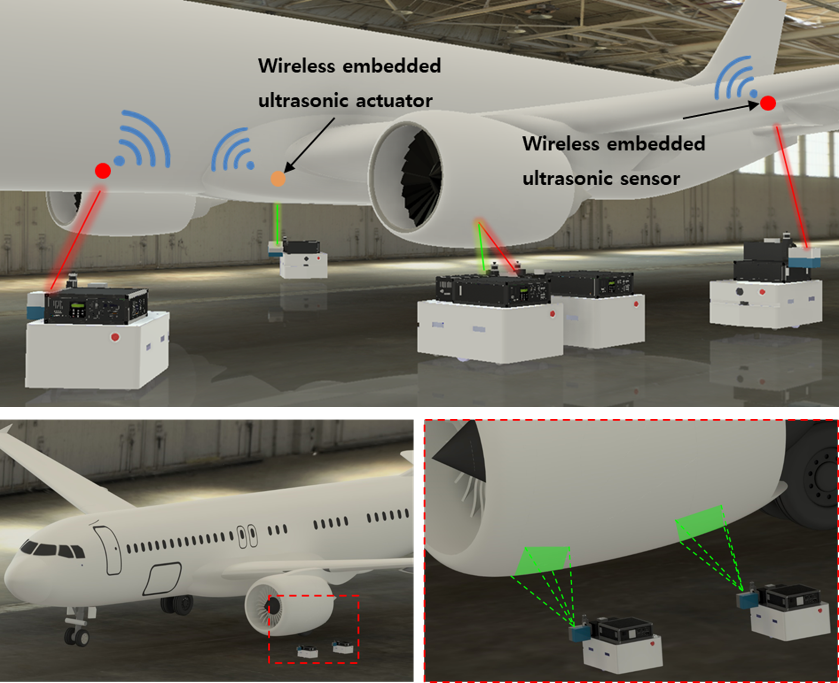
\includegraphics[width=\textwidth,keepaspectratio]{./images/rover_scan.png}
       \end{column}
    \end{columns}
\end{frame}

\section{System design}
\begin{frame}
  \vspace{1pt}
  {\LARGE{\text{\bf{System design}}}}
    \begin{columns}[T,onlytextwidth]
        \begin{column}{0.48\textwidth}
           \begin{itemize}
            \item Algorithmic Approach:
              \begin{itemize}
                \item Convex decomposition
                \item Morse decomposition
              \end{itemize}
            \item AI Model
              \begin{itemize}
                \item Q-Learning 
                \item DQN
                \item PPO
              \end{itemize}
           \end{itemize}

        \end{column}
        \begin{column}{0.48\textwidth}
            \centering
            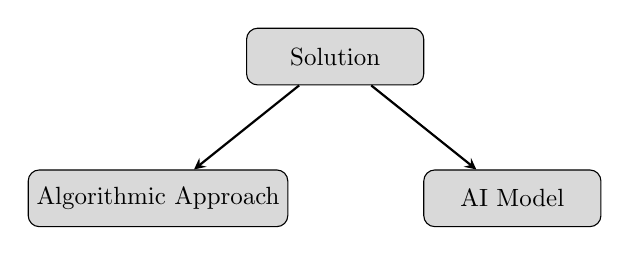
\begin{tikzpicture}[
                scale=0.9,
                transform shape,
                block/.style={
                    rectangle,
                    rounded corners,
                    minimum width=2.5cm,
                    minimum height=0.8cm,
                    text centered,
                    draw=black,
                    fill=gray!30
                },
                arrow/.style={thick, ->, >=stealth}
            ]

                \node[block] (sol) at (0,2) {Solution};
                \node[block] (alg) at (-2.5,0)
                    {Algorithmic Approach};
                \node[block] (ai) at (2.5,0)
                    {AI Model};

                \draw[arrow] (sol) -- (alg);
                \draw[arrow] (sol) -- (ai);

            \end{tikzpicture}

            \medskip
            {\scriptsize
            Possible approaches to solving the problem}
        \end{column}
    \end{columns}
\end{frame}

\section{Communication architecture}
\begin{frame}
  \vspace{1pt}
  {\LARGE\bf{Communication architecture}}
  \begin{figure}[htbp]
  \centering
    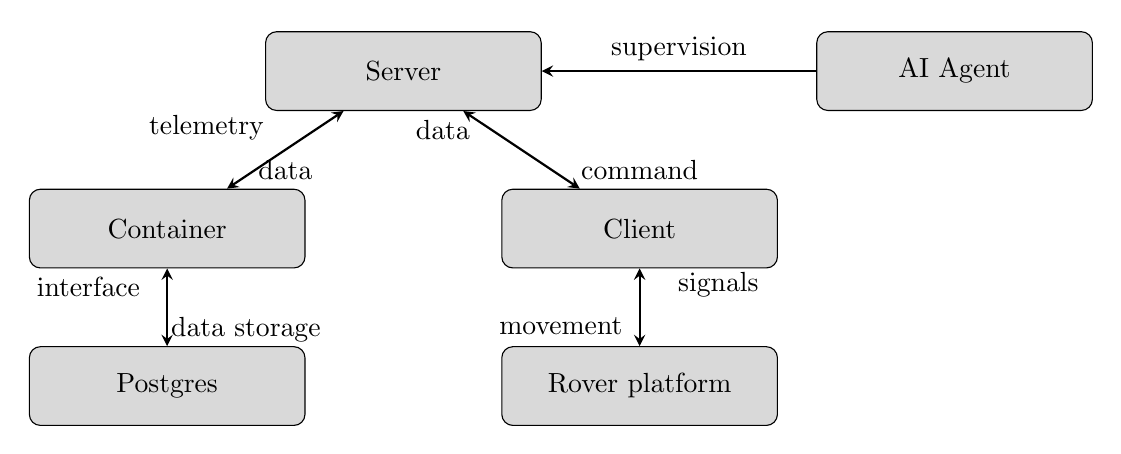
\begin{tikzpicture}[block/.style={rectangle, rounded corners, minimum width=3.5cm, minimum height=1cm, text centered, draw=black, fill=gray!30}, arrow/.style={thick, ->, >=stealth}, arrow2/.style={thick, <->, >=stealth}]

      \node[block] (agent) at (7,2) {AI Agent};
      \node[block] (server) at (0,2) {Server};

      \node[block] (con) at (-3,0) {Container};
      \node[block] (post) at (-3,-2) {Postgres};

      \node[block] (client) at (3,0) {Client};
      \node[block] (rover) at (3,-2) {Rover platform};

      \draw[arrow] (agent) -- node[above] {supervision} (server);
      \draw[arrow2] (server) -- node[below] {data} node[above, xshift = -10mm] {telemetry} (con);
      \draw[arrow2] (server) -- node[above, xshift = -10mm] {data} node[below, xshift = 15mm] {command} (client);

      \draw[arrow2] (client) -- node[below, xshift = -10mm] {movement} node[above, xshift=10mm] {signals} (rover);
      \draw[arrow2] (con) -- node[above, xshift = -10mm] {interface} node[below, xshift = 10mm] {data storage} (post);

    \end{tikzpicture}
  \end{figure}
\end{frame}

\section{AI development}
\begin{frame}
  \vspace{10pt}
  {\LARGE\bf{AI development}}
  \begin{figure}
    \centering
    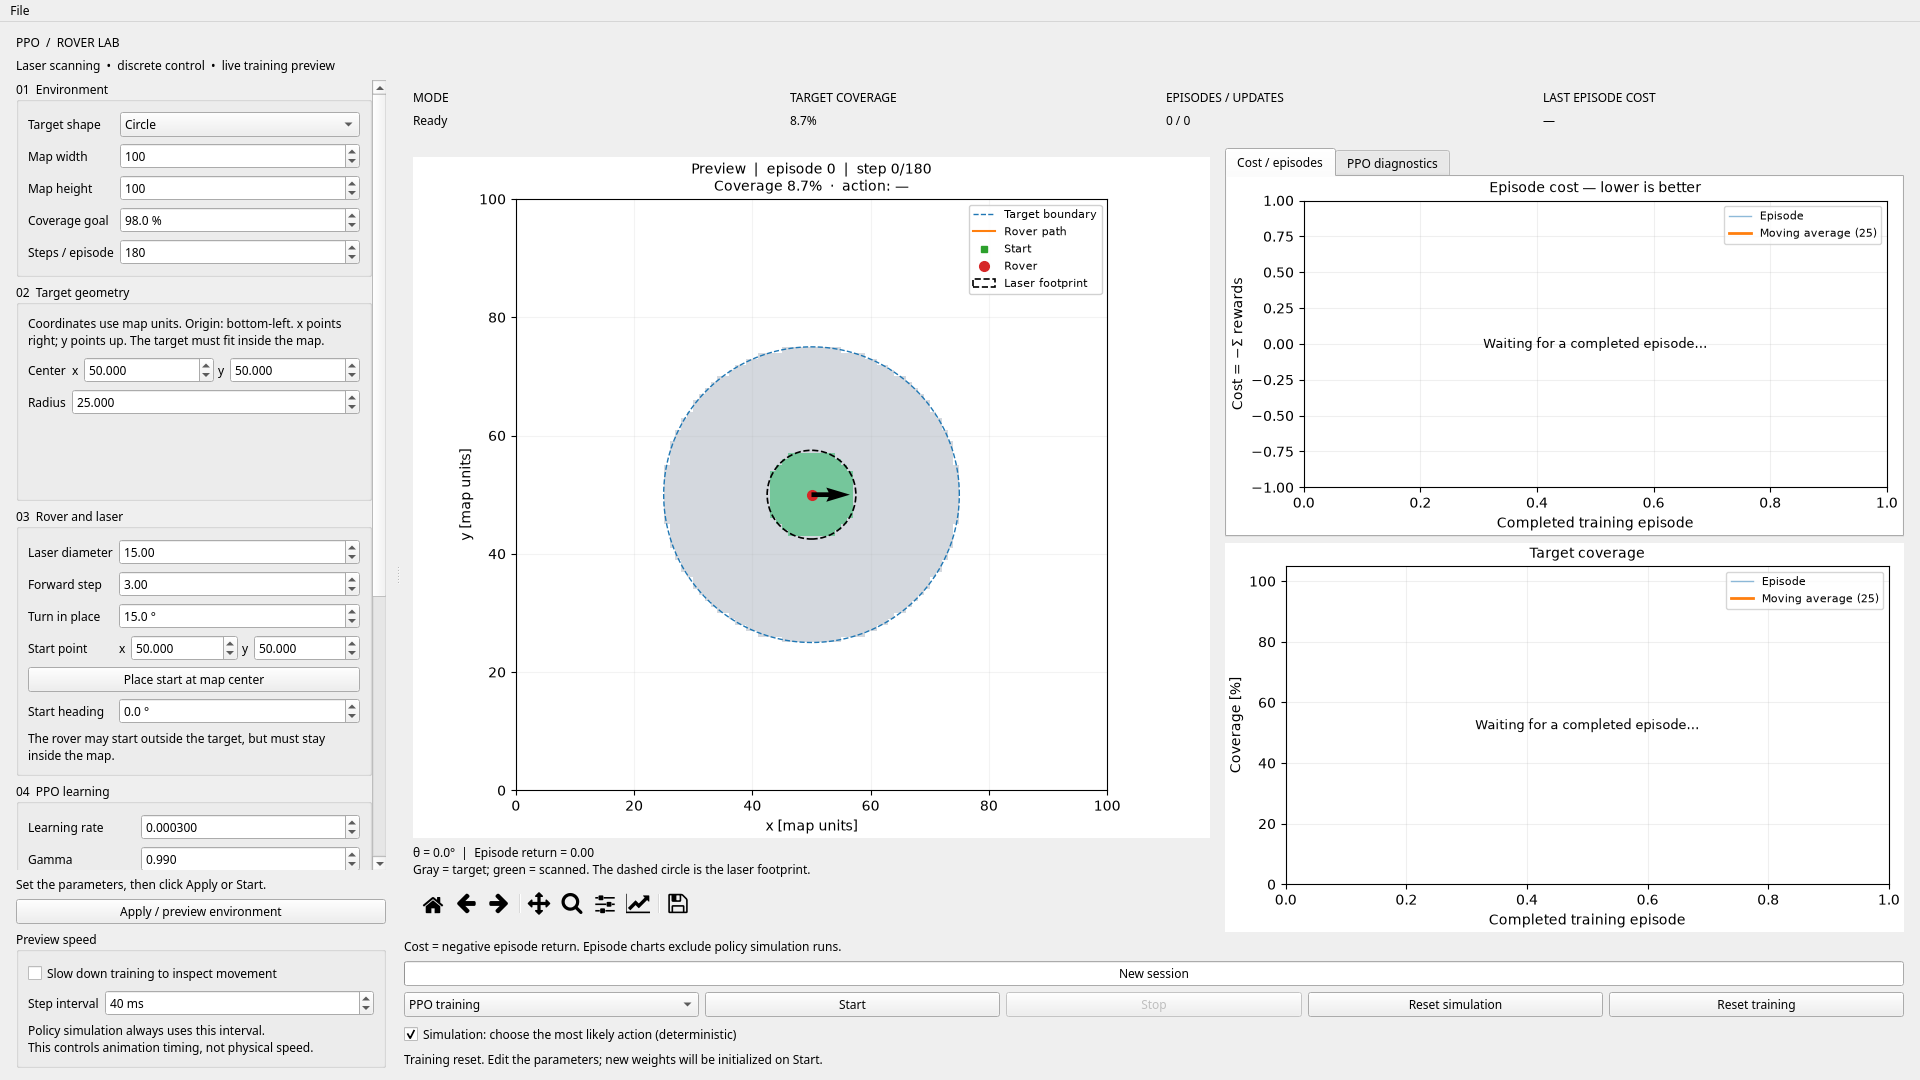
\includegraphics[width=0.75\textwidth,keepaspectratio]{../images/simulation.png}
  \end{figure}
\end{frame}

\begin{frame}
  \vspace{20pt}
  {\LARGE\bf{AI training with circle}}
  \begin{table}
    \begin{tabular}{|l|l|l|}
      \hline
      1. & envinronment dimentions & $ 150 \times 150 $  \\
      \hline
      2. & center of the circle & $ (75, 75) $  \\
      \hline
      3. & circle radius & 25  \\
      \hline
      4. & rover starting point & $ (50, 50) $  \\
      \hline
    \end{tabular}
  \end{table}

  \begin{figure}
    \centering
    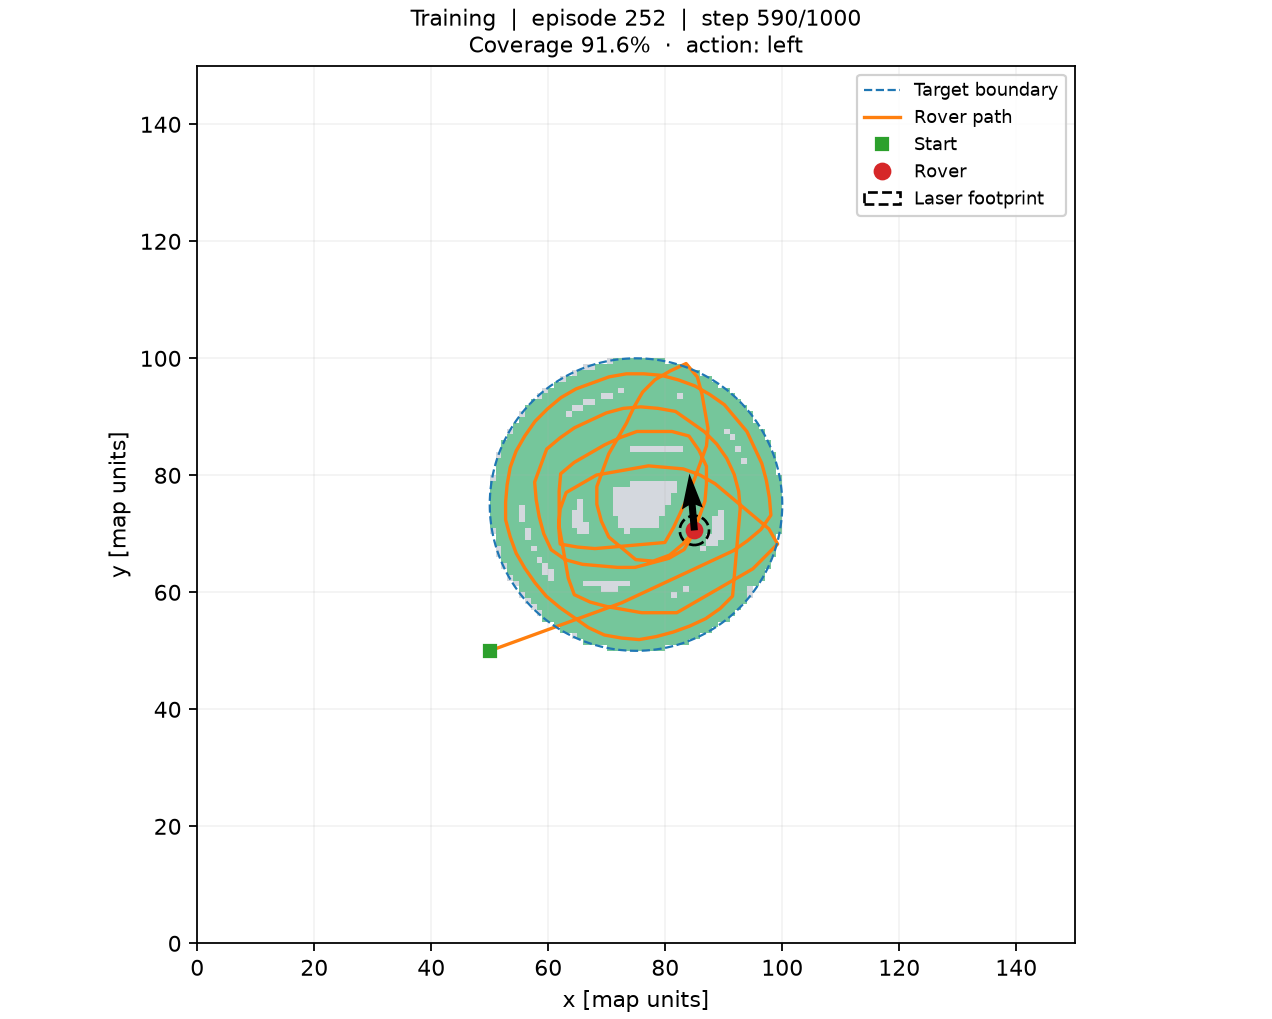
\includegraphics[width=0.32\textwidth,keepaspectratio]{../images/circle_250episodes/rover.png}
    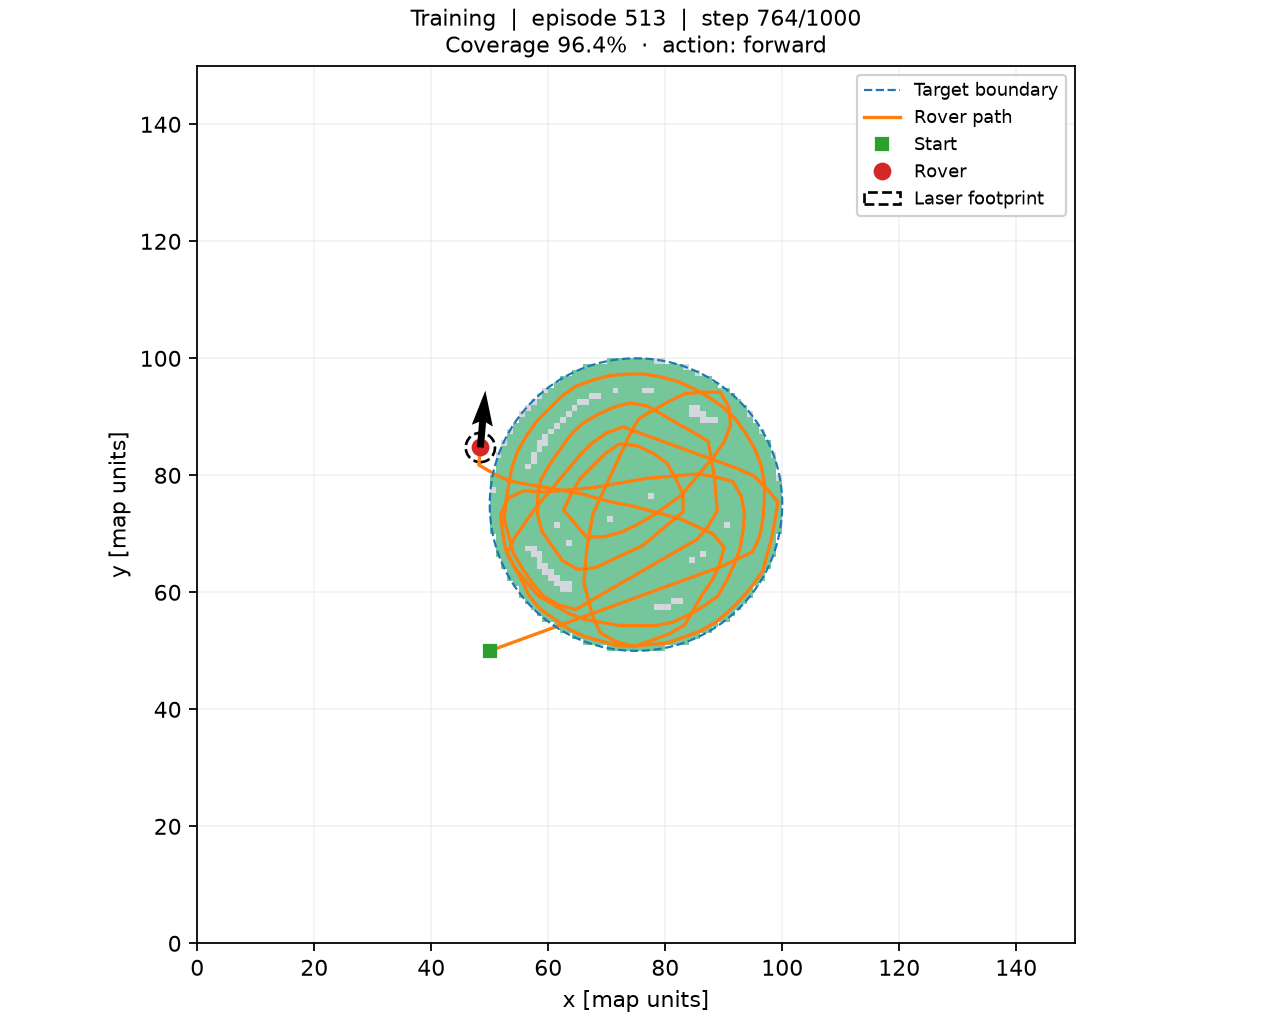
\includegraphics[width=0.32\textwidth,keepaspectratio]{../images/circle_500episodes/rover.png}
    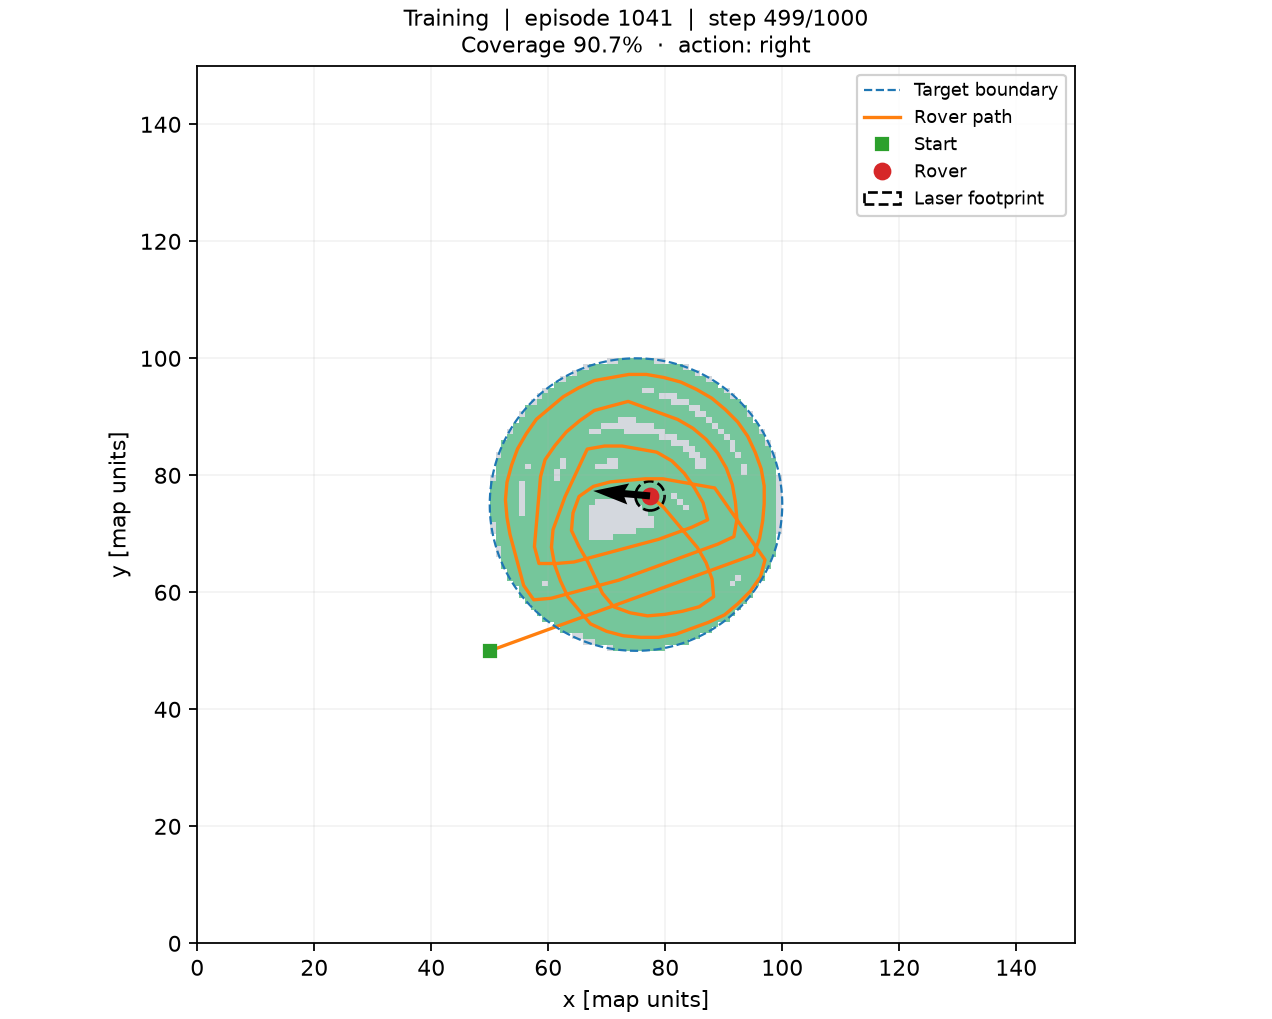
\includegraphics[width=0.32\textwidth,keepaspectratio]{../images/circle_1000episodes/rover.png}
    \caption{Training results after 250, 500, 1000 episodes}
  \end{figure}
\end{frame}

\begin{frame}
  \vspace{20pt}
  {\LARGE\bf{AI training with triangle}}
\begin{table}
  \begin{tabular}{|l|l|l|}
    \hline
    1. & environment dimentions & $ 150 \times 150 $  \\
    \hline
    2. & triangle verticies & $ (40, 90), (100, 30), (100, 90) $  \\
    \hline
    3. & rover starting point & $ (50, 50) $  \\
    \hline
  \end{tabular}
\end{table}


  \begin{figure}
    \centering
    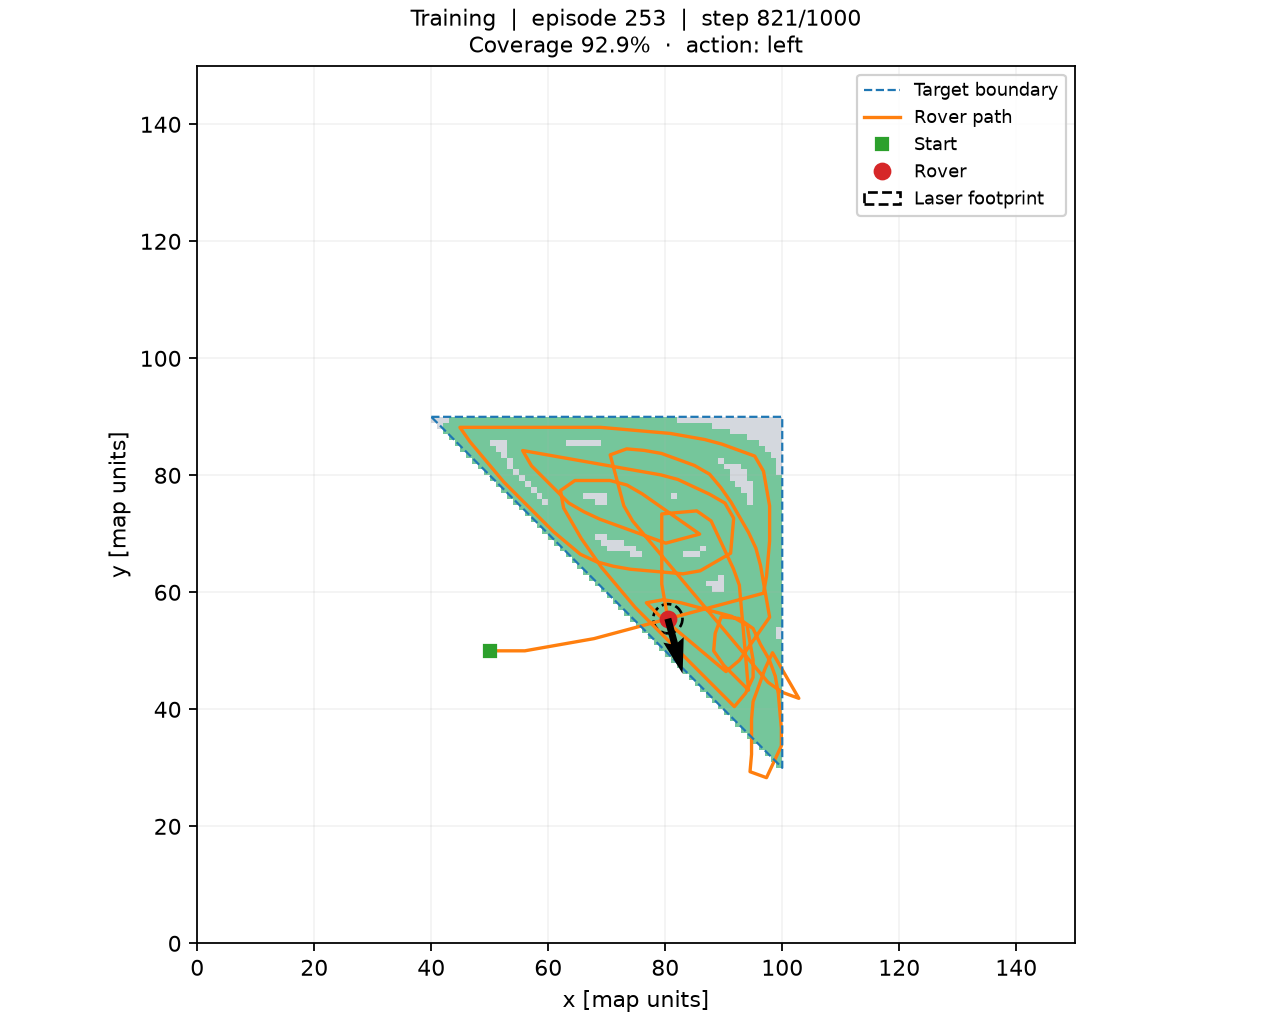
\includegraphics[width=0.32\textwidth,keepaspectratio]{../images/triangle_250episodes/rover.png}
    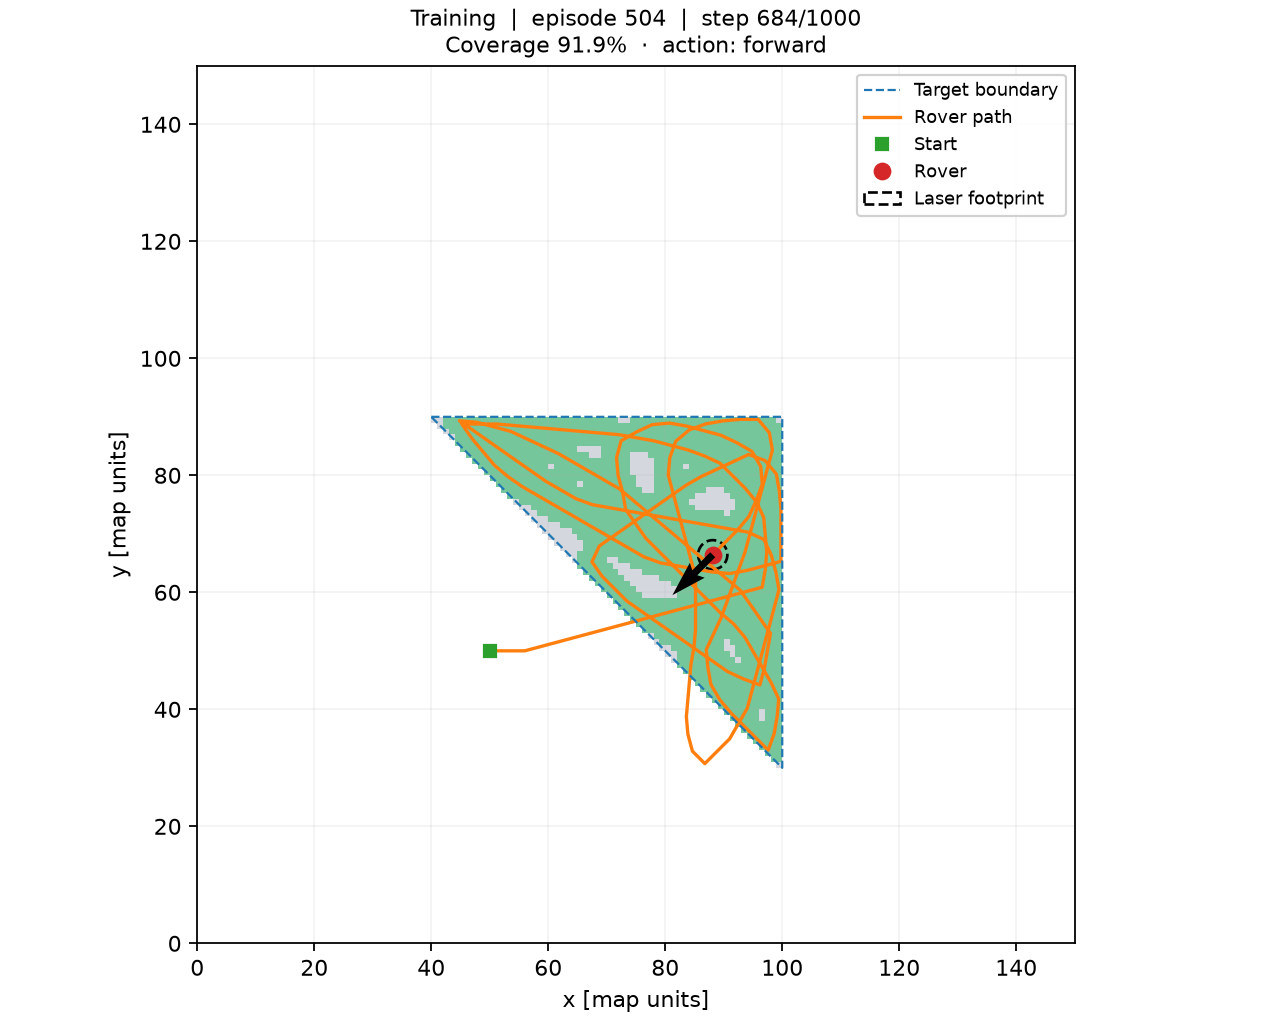
\includegraphics[width=0.32\textwidth,keepaspectratio]{../images/triangle_500episodes/rover.png}
    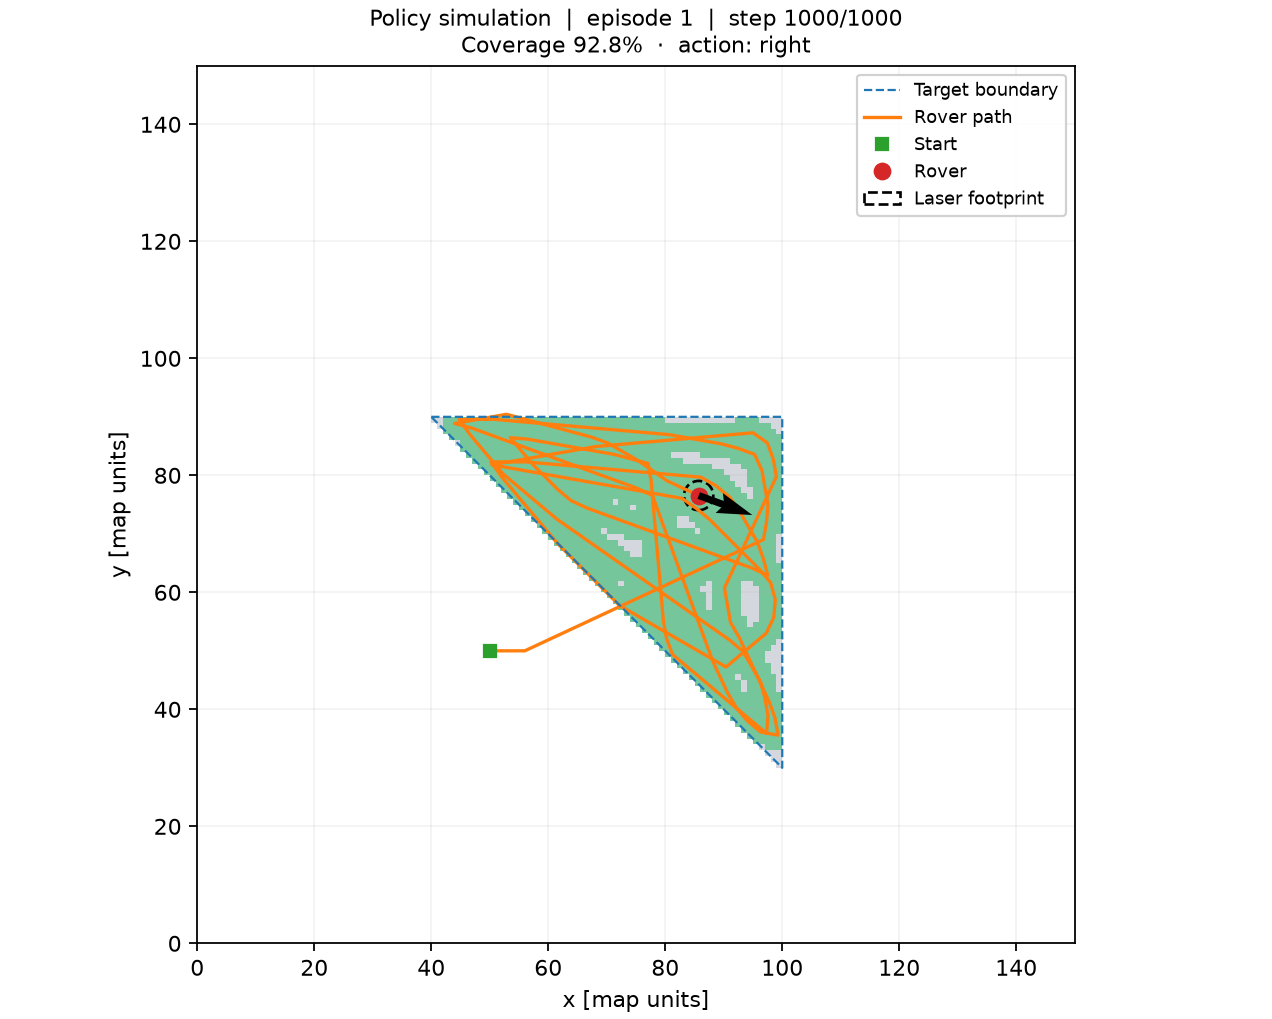
\includegraphics[width=0.32\textwidth,keepaspectratio]{../images/triangle_1000episodes/rover.png}
    \caption{Training results after 250, 500, 1000 episodes}
  \end{figure}
\end{frame}

\begin{frame}
  \vspace{10pt}
  {\LARGE\bf{AI training with ellipse}}
  \begin{table}
  \begin{tabular}{|l|l|l|}
    \hline
    1. & environment dimensions & $ 150 \times 150 $  \\
    \hline
    2. & semi-major axis & 30  \\
    \hline
    3. & semi-minor axis & 20  \\
    \hline
    4. & center of the ellipse & $ (70, 100) $  \\
    \hline
    5. & rover starting point & $ (50, 50) $  \\
    \hline
  \end{tabular}
  \end{table}

  \begin{figure}
    \centering
    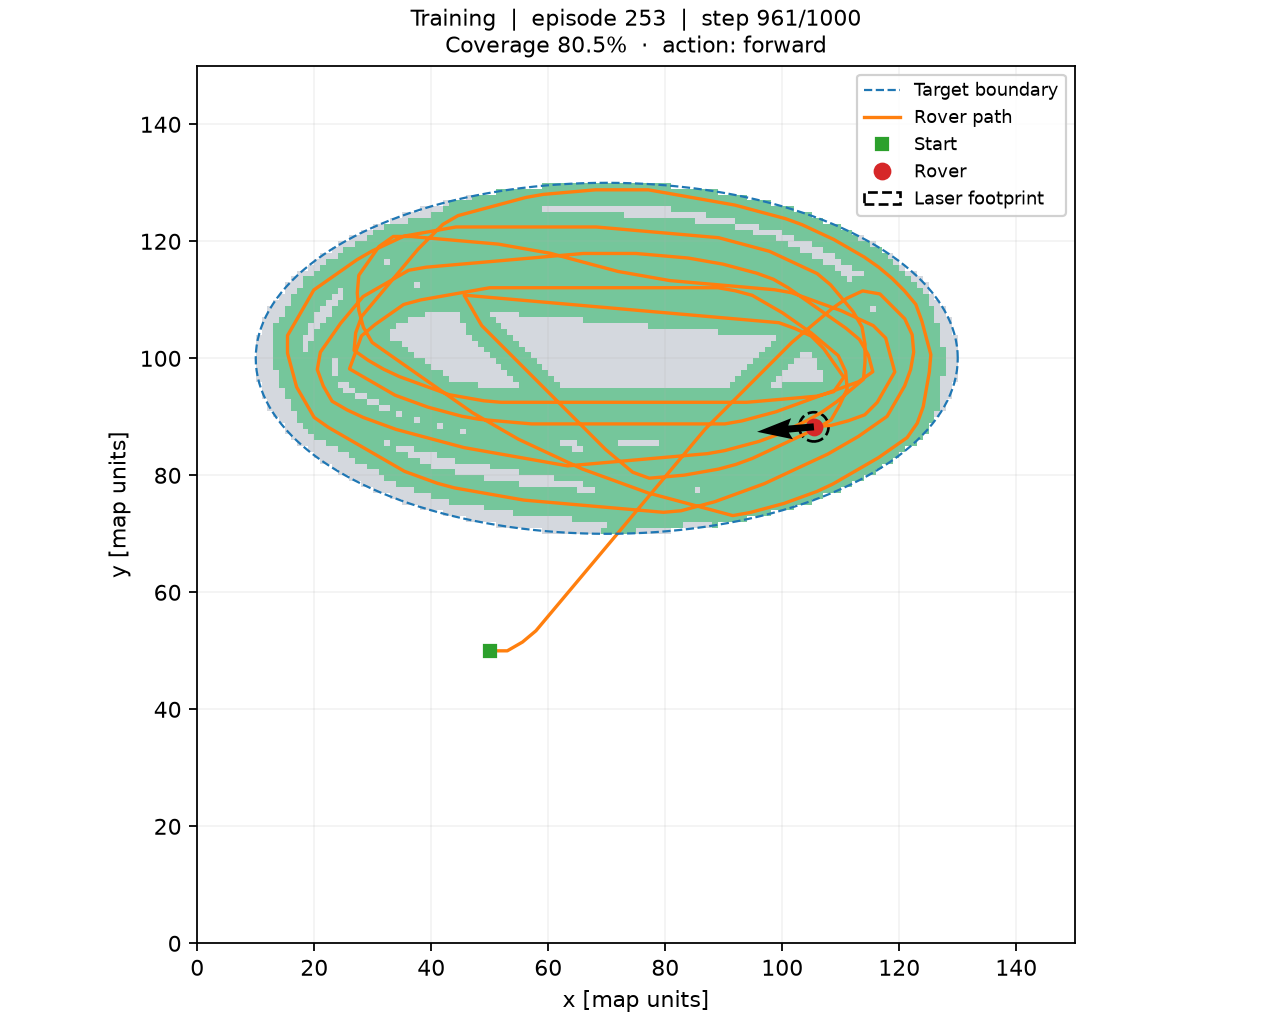
\includegraphics[width=0.32\textwidth,keepaspectratio]{../images/ellipse_250episodes/rover.png}
    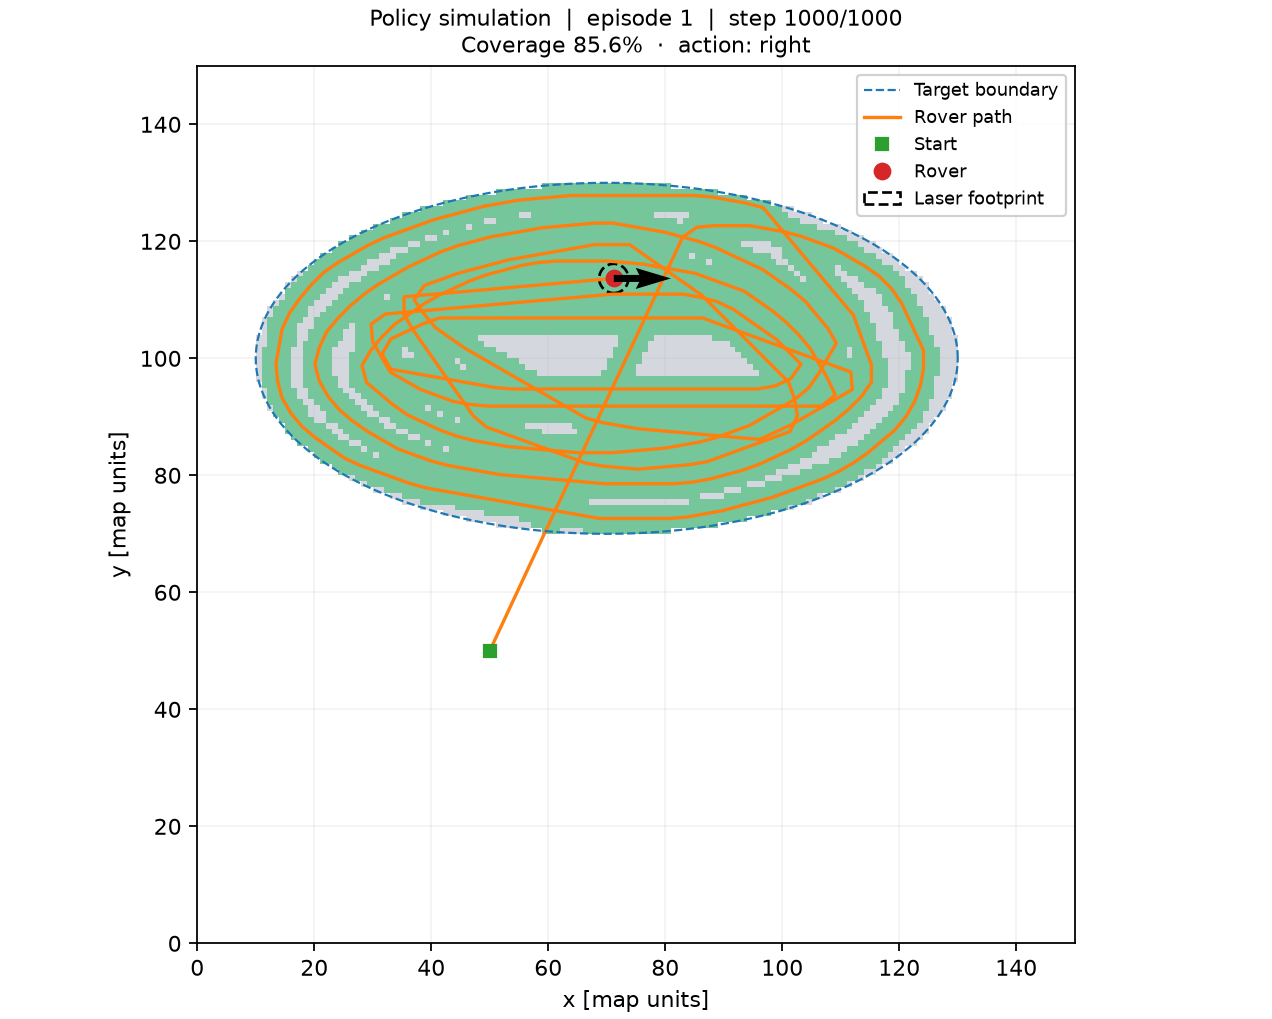
\includegraphics[width=0.32\textwidth,keepaspectratio]{../images/ellipse_500episodes/rover.png}
    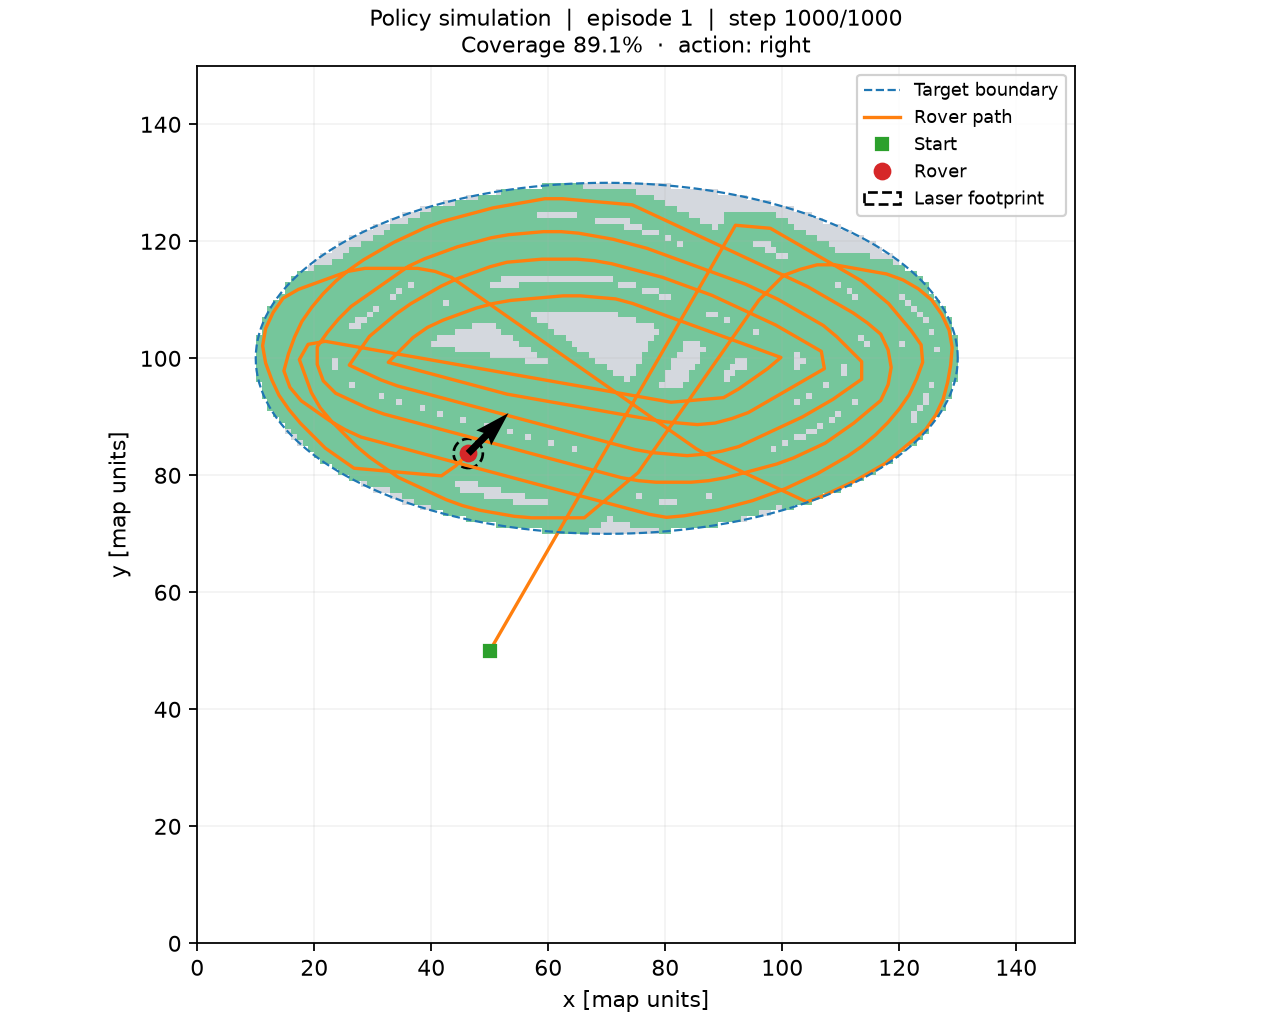
\includegraphics[width=0.32\textwidth,keepaspectratio]{../images/ellipse_1000episodes/rover.png}
    \caption{Training results after 250, 500, 1000 episodes}
  \end{figure}
\end{frame}

\begin{frame}
  \vspace{20pt}
  {\LARGE\bf{Srface coverage comparison}}
  \begin{figure}
    \centering
    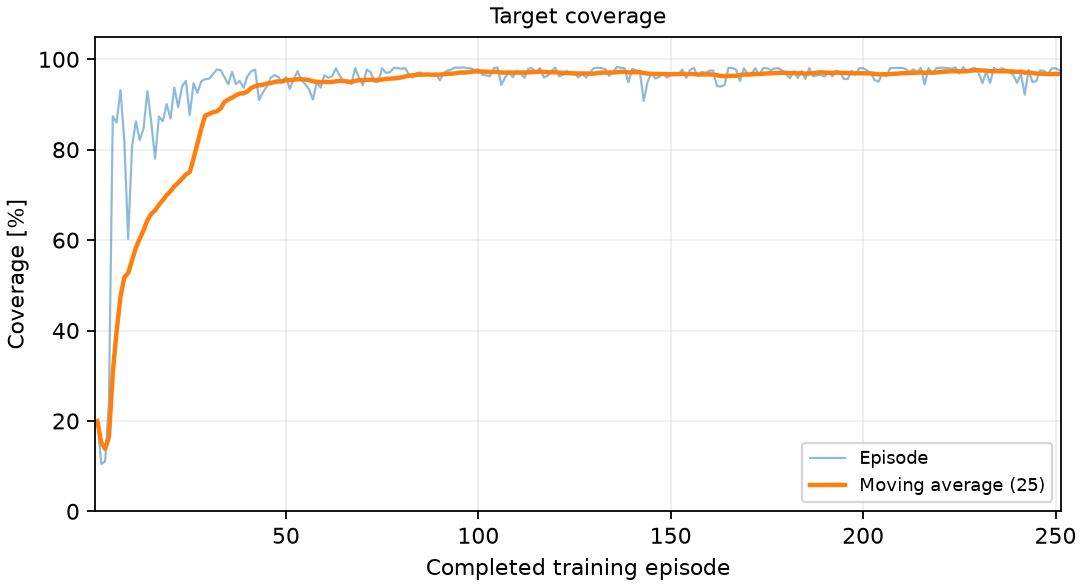
\includegraphics[width=0.32\textwidth,keepaspectratio]{../images/circle_250episodes/coverage.png}
    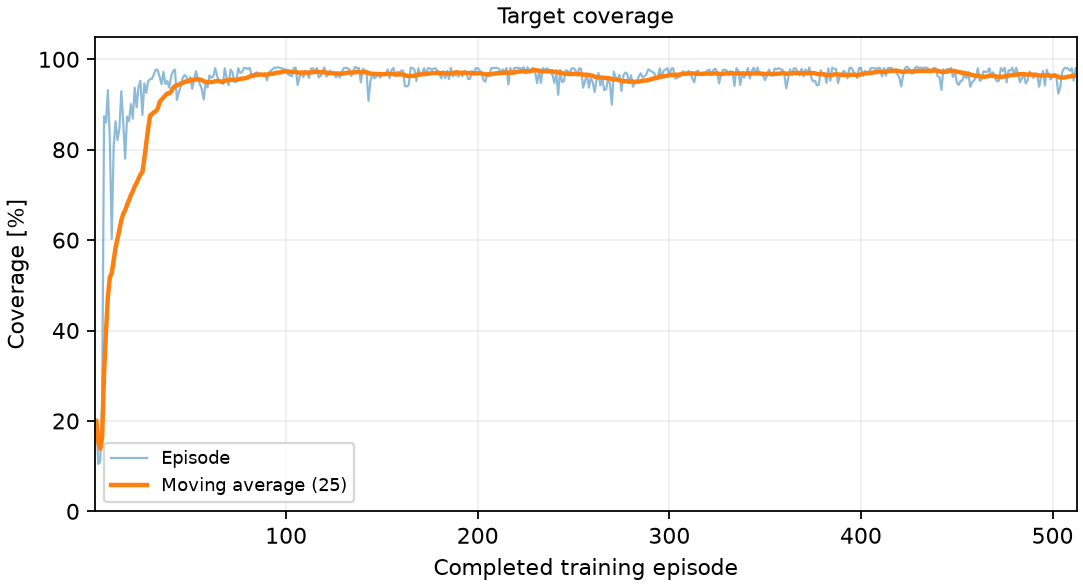
\includegraphics[width=0.32\textwidth,keepaspectratio]{../images/circle_500episodes/coverage.png}
    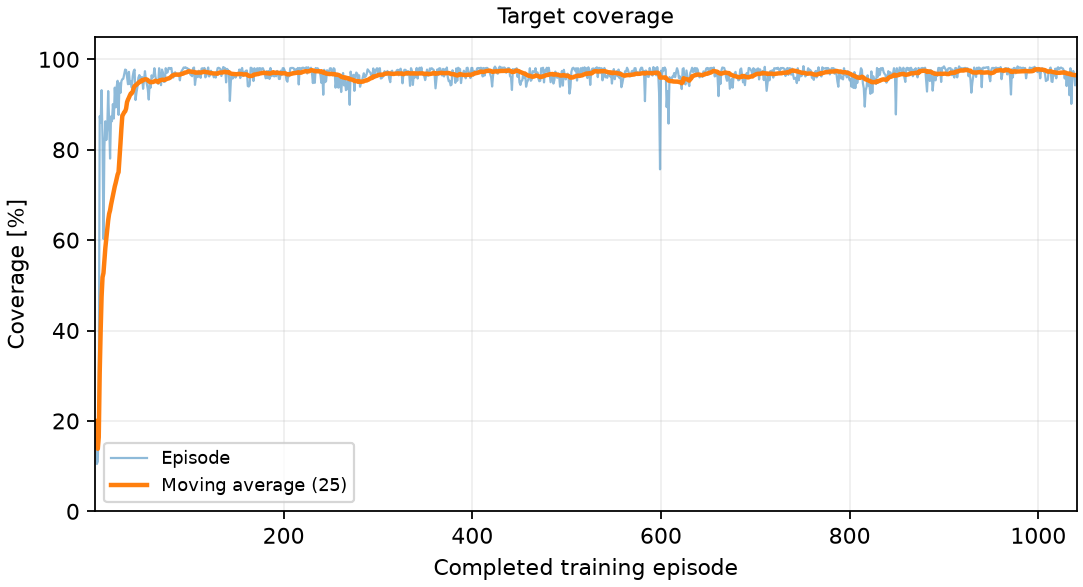
\includegraphics[width=0.32\textwidth,keepaspectratio]{../images/circle_1000episodes/coverage.png}

    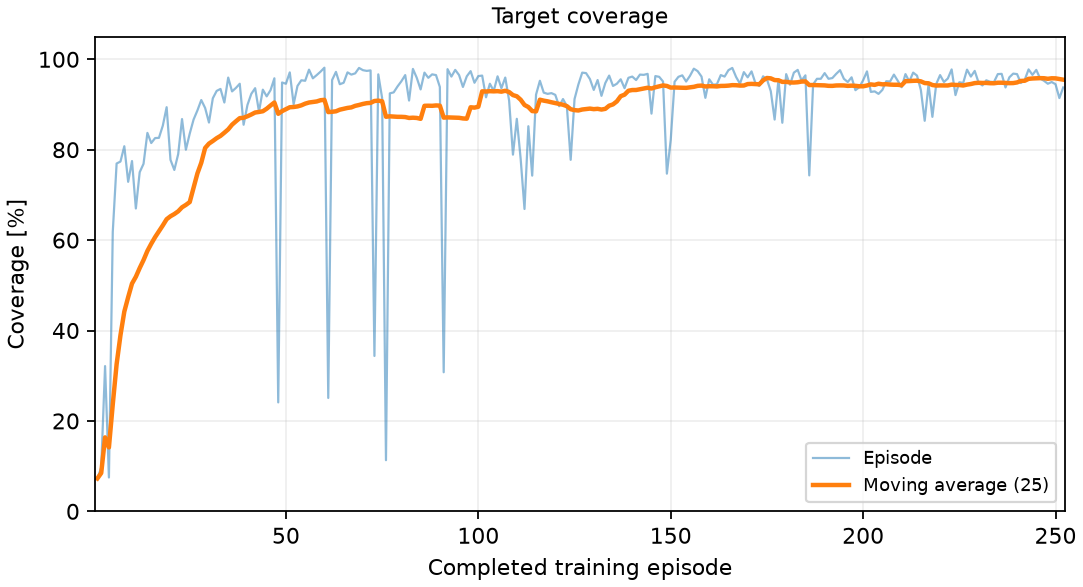
\includegraphics[width=0.32\textwidth,keepaspectratio]{../images/triangle_250episodes/coverage.png}
    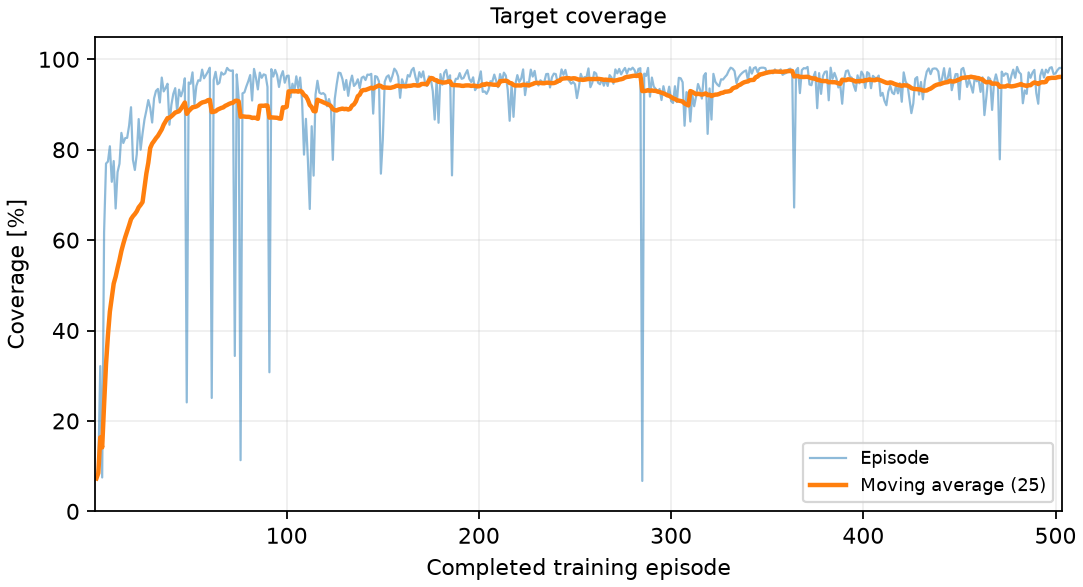
\includegraphics[width=0.32\textwidth,keepaspectratio]{../images/triangle_500episodes/coverage.png}
    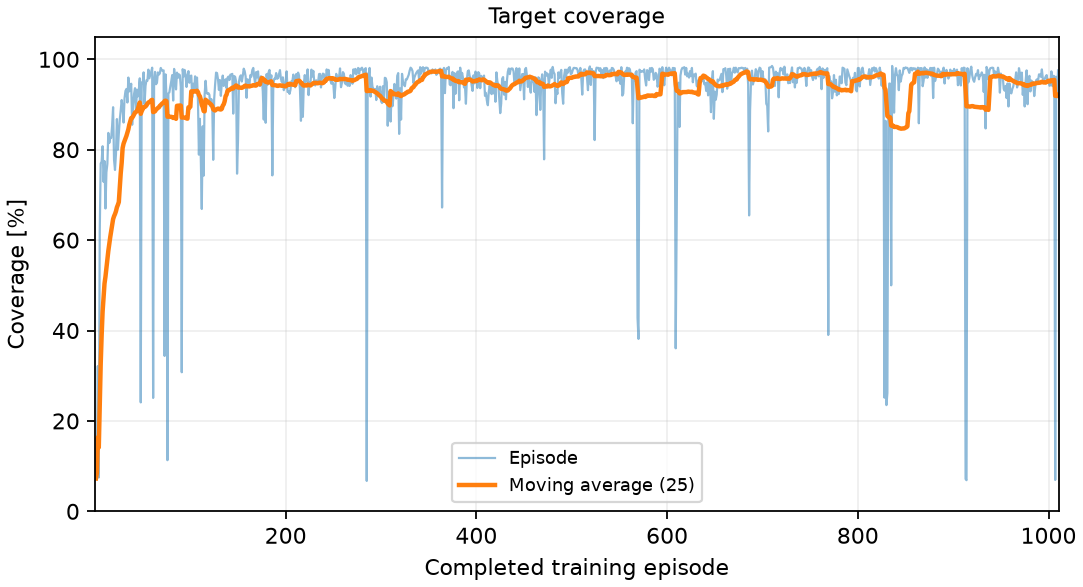
\includegraphics[width=0.32\textwidth,keepaspectratio]{../images/triangle_1000episodes/coverage.png}

    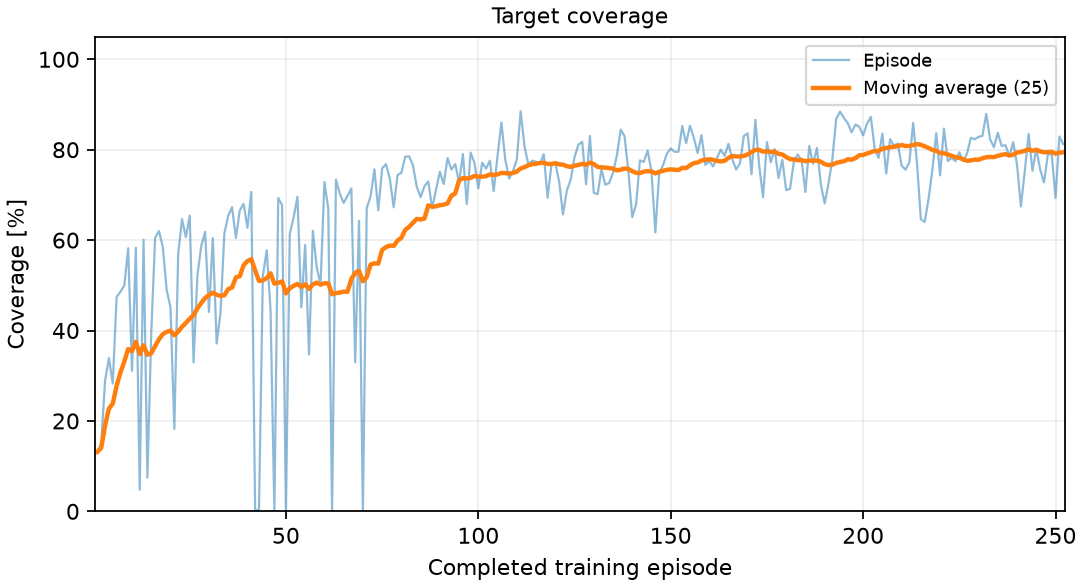
\includegraphics[width=0.32\textwidth,keepaspectratio]{../images/ellipse_250episodes/coverage.png}
    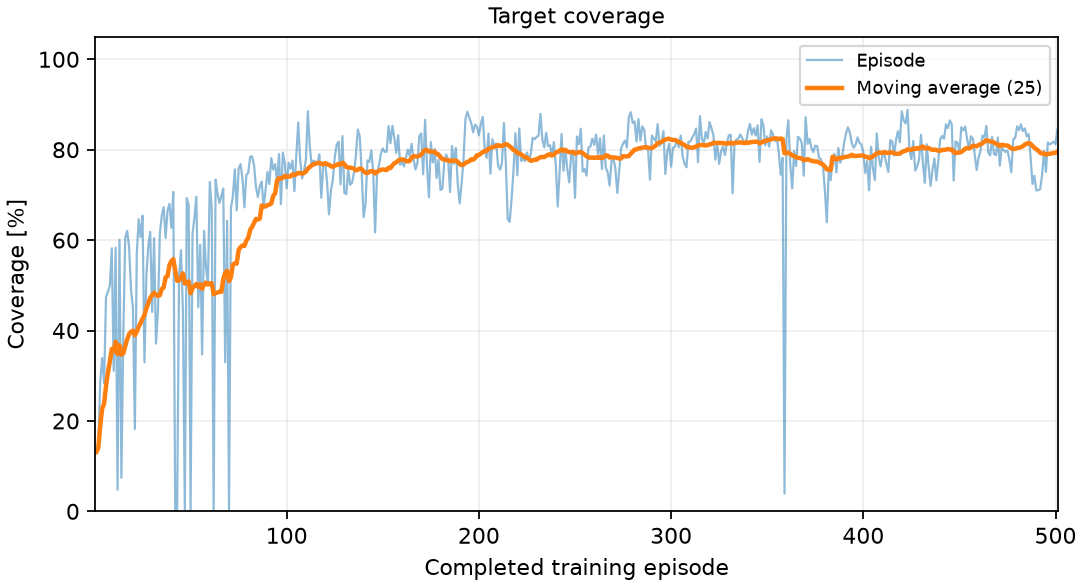
\includegraphics[width=0.32\textwidth,keepaspectratio]{../images/ellipse_500episodes/coverage.png}
    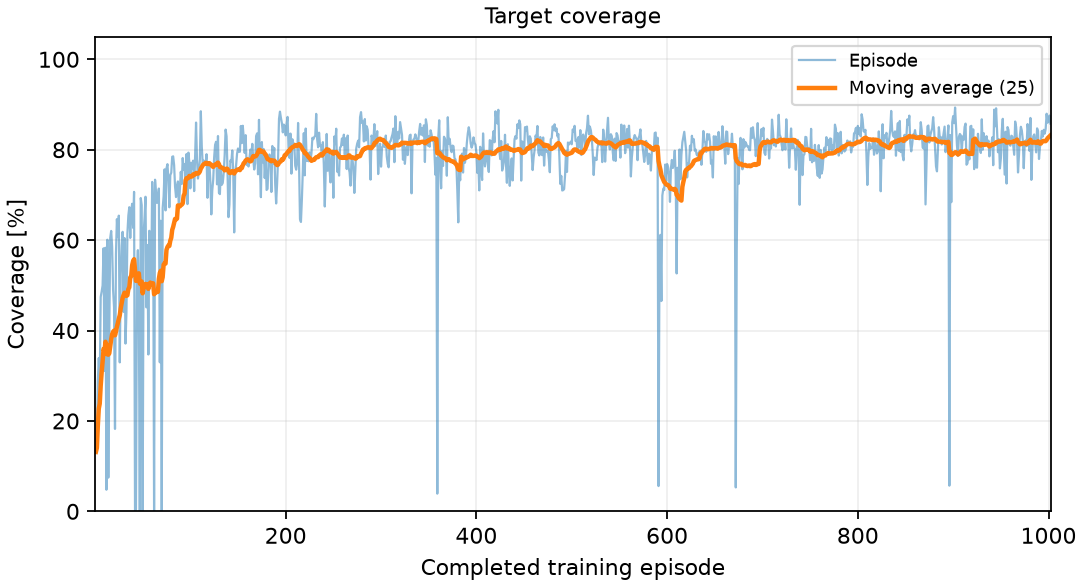
\includegraphics[width=0.32\textwidth,keepaspectratio]{../images/ellipse_1000episodes/coverage.png}
  \end{figure}
\end{frame}

\begin{frame}
  \vspace{20pt}
  {\LARGE\bf{Episode cost comparison}}
  \begin{figure}
    \centering
    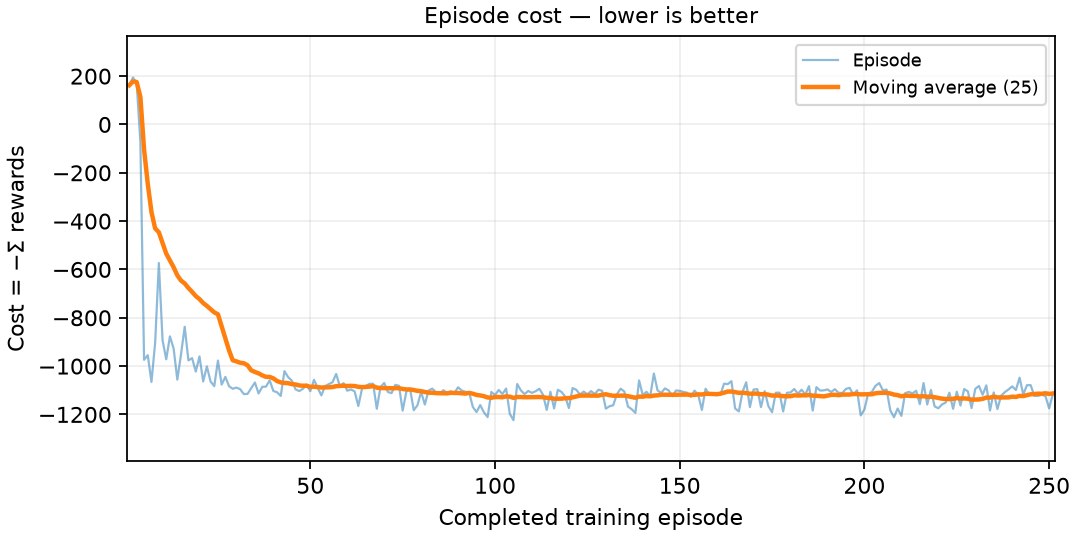
\includegraphics[width=0.32\textwidth,keepaspectratio]{../images/circle_250episodes/episode_cost.png}
    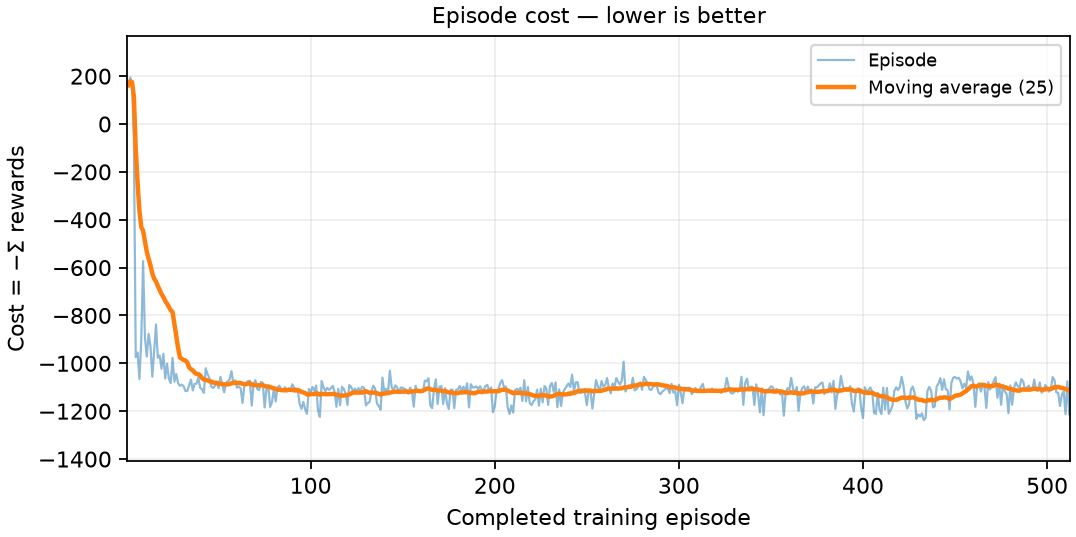
\includegraphics[width=0.32\textwidth,keepaspectratio]{../images/circle_500episodes/episode_cost.png}
    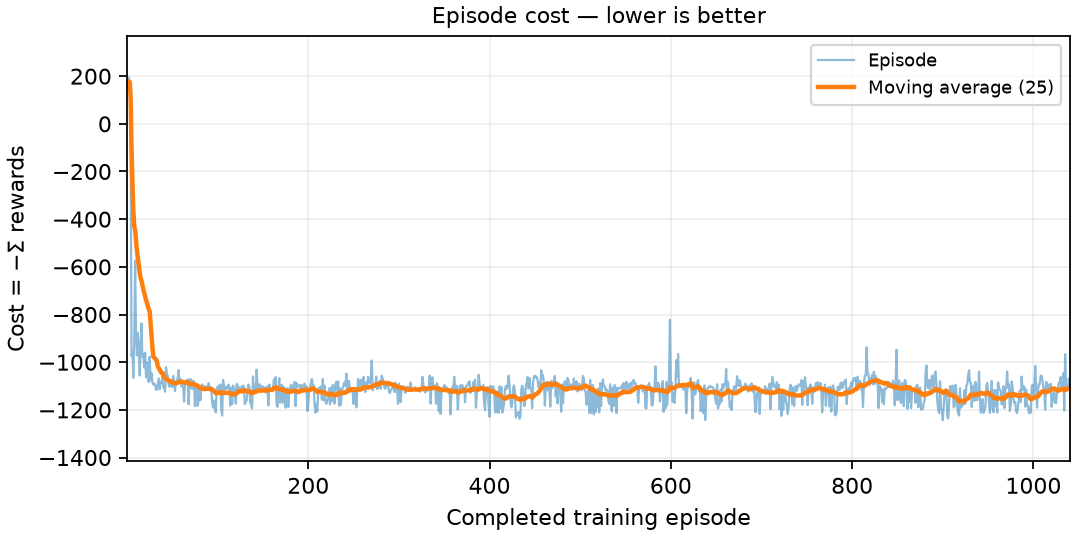
\includegraphics[width=0.32\textwidth,keepaspectratio]{../images/circle_1000episodes/episode_cost.png}

    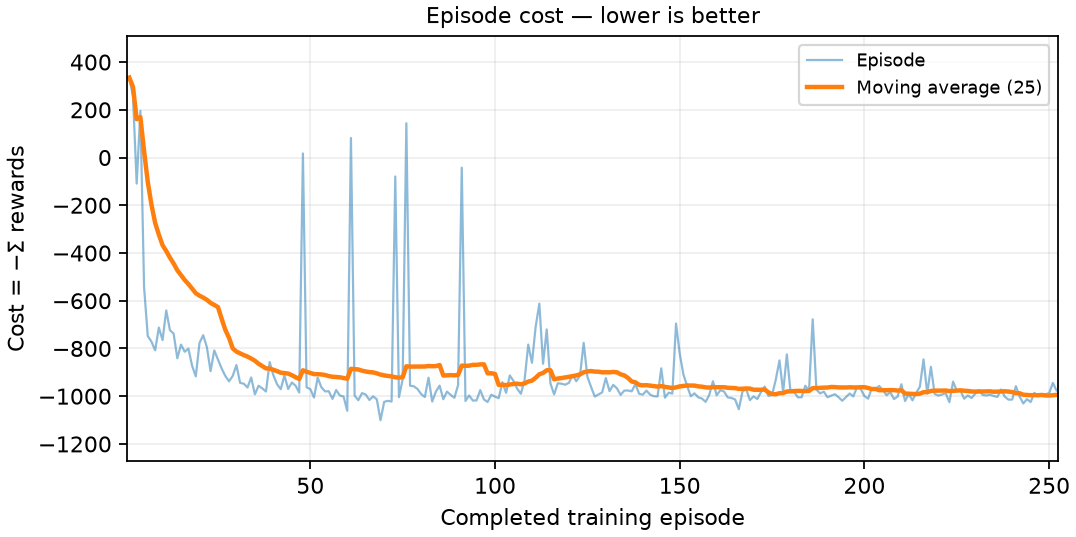
\includegraphics[width=0.32\textwidth,keepaspectratio]{../images/triangle_250episodes/episode_cost.png}
    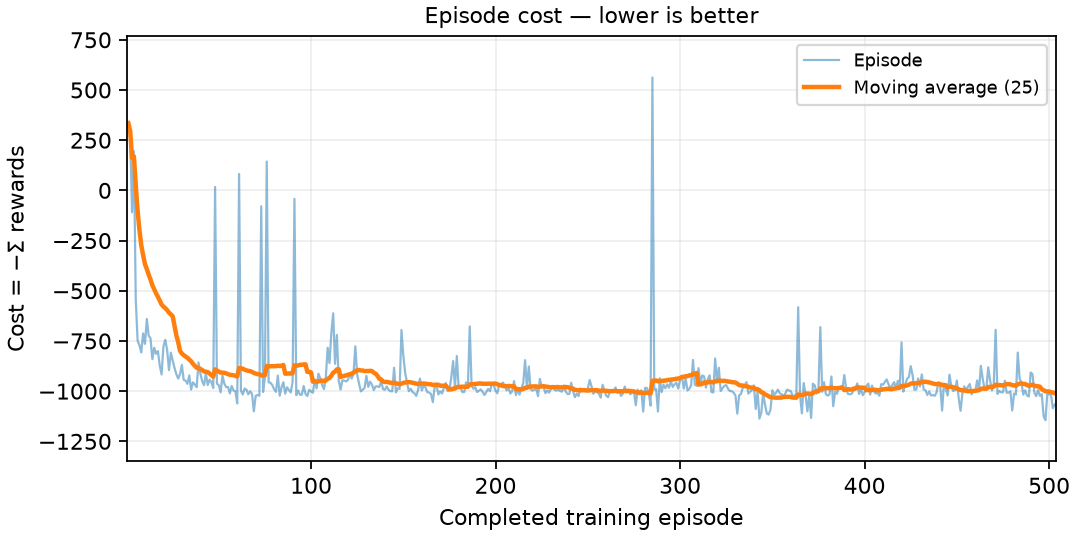
\includegraphics[width=0.32\textwidth,keepaspectratio]{../images/triangle_500episodes/episode_cost.png}
    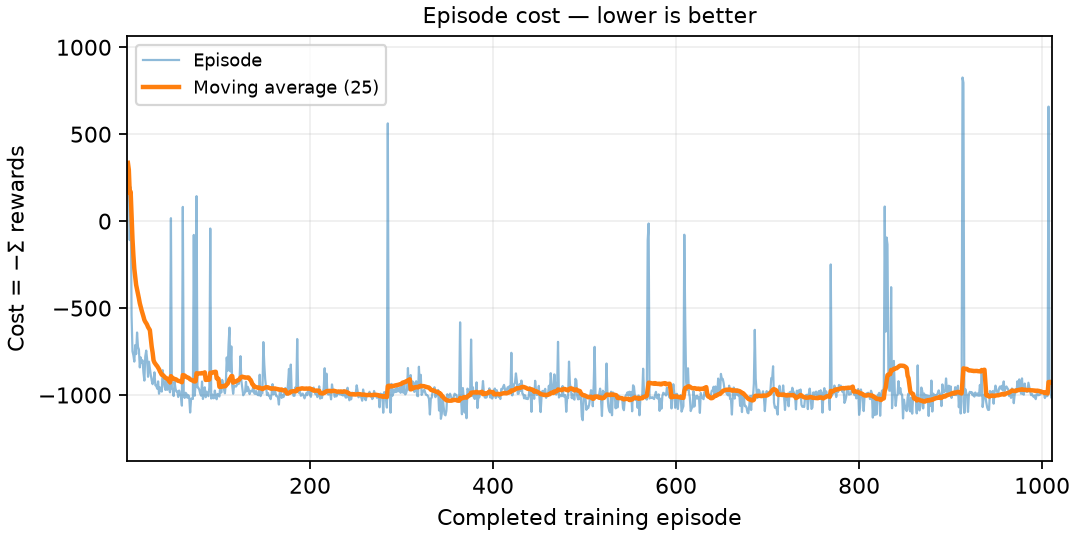
\includegraphics[width=0.32\textwidth,keepaspectratio]{../images/triangle_1000episodes/episode_cost.png}

    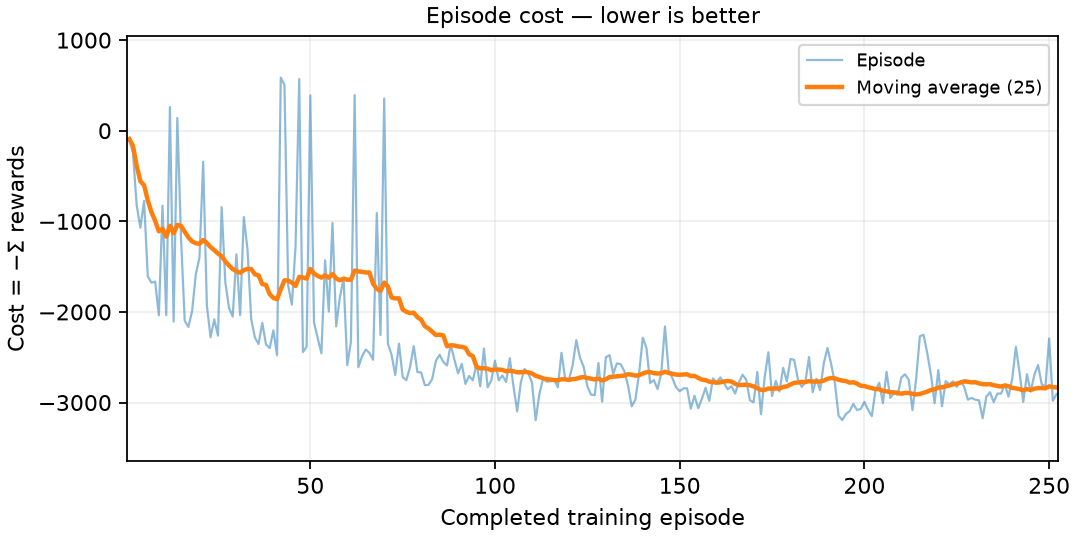
\includegraphics[width=0.32\textwidth,keepaspectratio]{../images/ellipse_250episodes/episode_cost.png}
    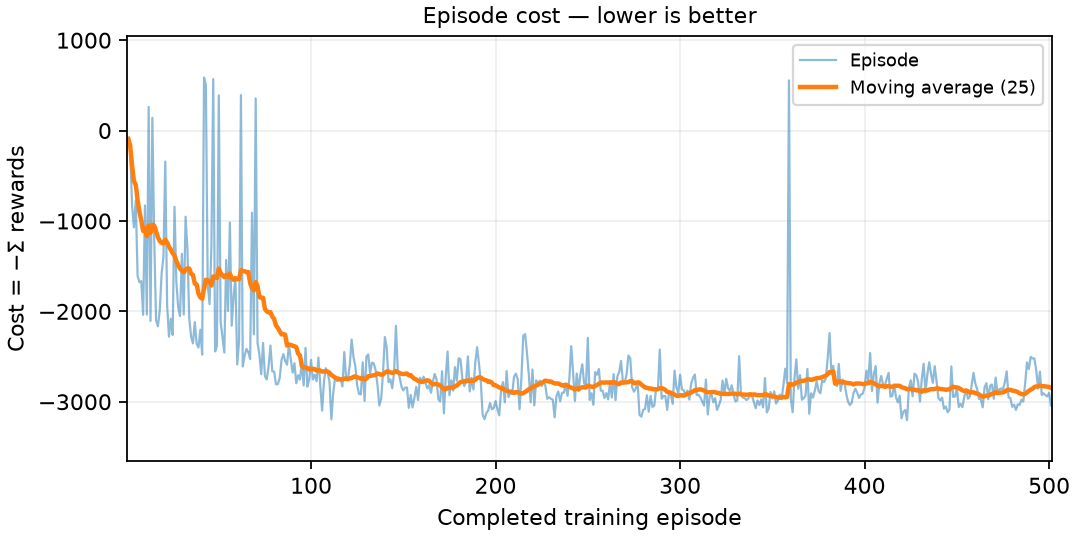
\includegraphics[width=0.32\textwidth,keepaspectratio]{../images/ellipse_500episodes/episode_cost.png}
    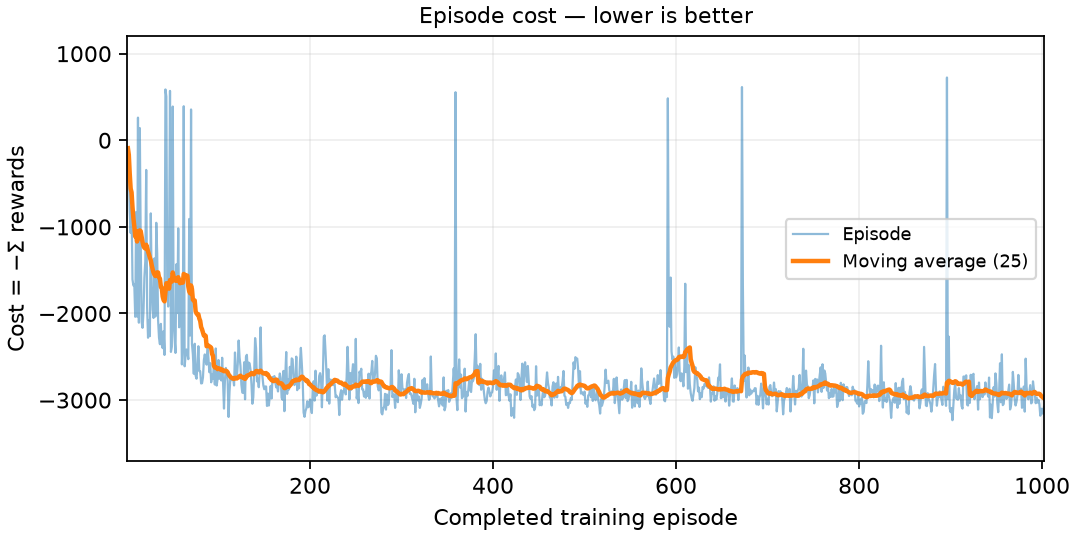
\includegraphics[width=0.32\textwidth,keepaspectratio]{../images/ellipse_1000episodes/episode_cost.png}
  \end{figure}
\end{frame}

\begin{frame}
  \vspace{20pt}
  {\LARGE\bf{PPO loss comparison}}
  \begin{figure}
    \centering
    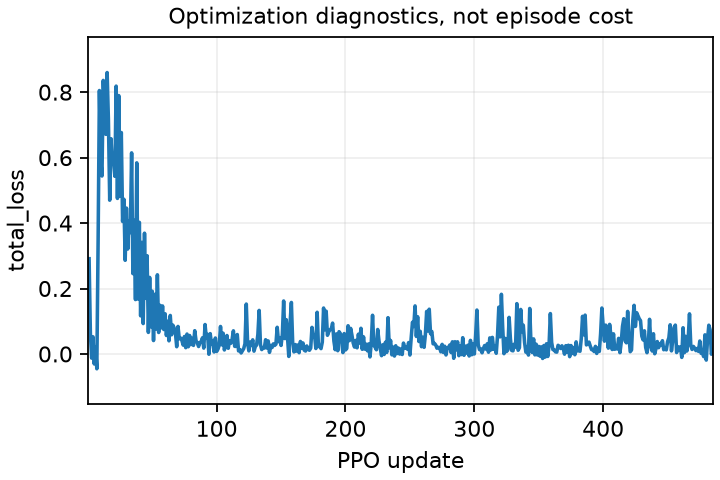
\includegraphics[width=0.25\textwidth,keepaspectratio]{../images/circle_250episodes/ppo_loss.png}
    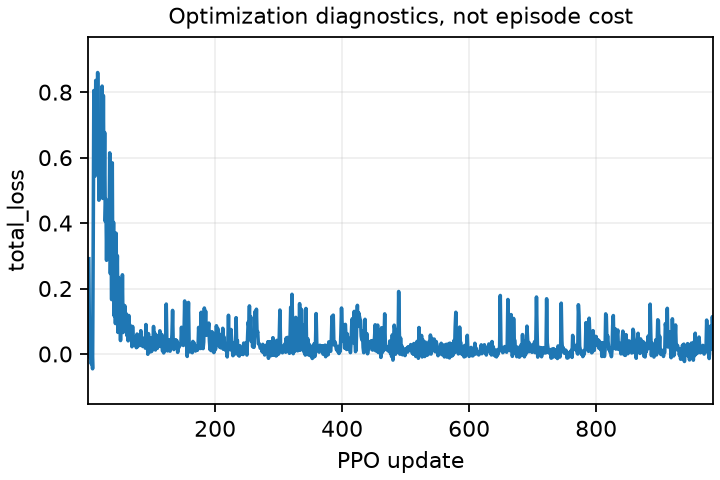
\includegraphics[width=0.25\textwidth,keepaspectratio]{../images/circle_500episodes/ppo_loss.png}
    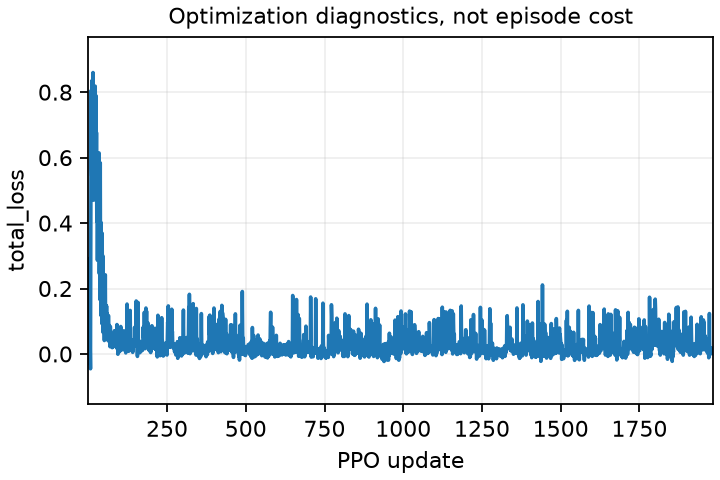
\includegraphics[width=0.25\textwidth,keepaspectratio]{../images/circle_1000episodes/ppo_loss.png}

    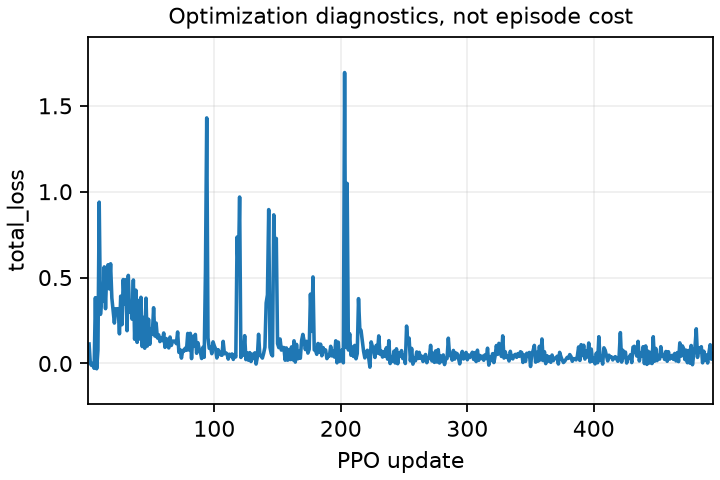
\includegraphics[width=0.25\textwidth,keepaspectratio]{../images/triangle_250episodes/ppo_loss.png}
    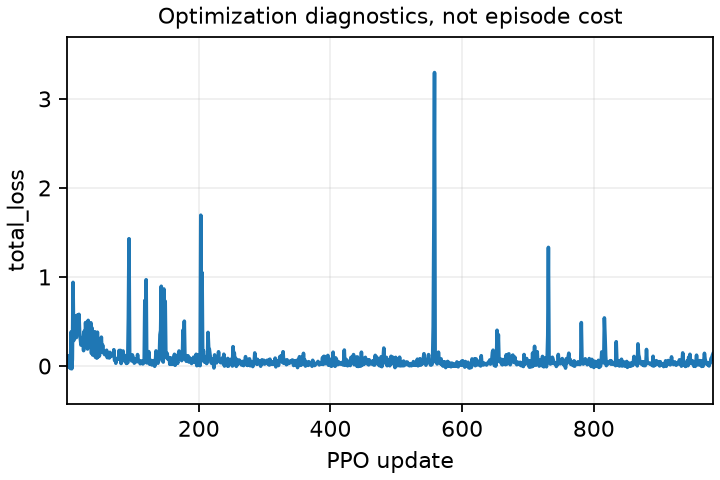
\includegraphics[width=0.25\textwidth,keepaspectratio]{../images/triangle_500episodes/ppo_loss.png}
    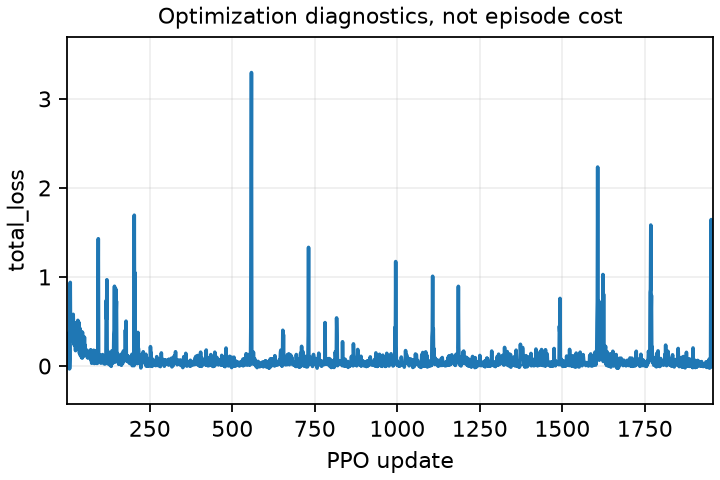
\includegraphics[width=0.25\textwidth,keepaspectratio]{../images/triangle_1000episodes/ppo_loss.png}

    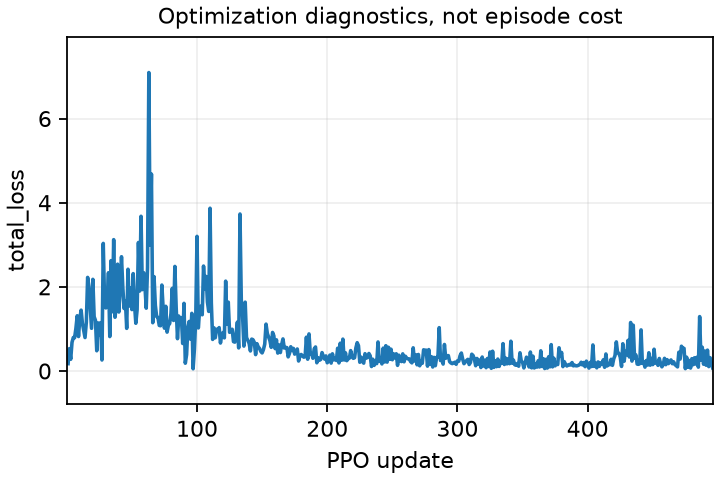
\includegraphics[width=0.25\textwidth,keepaspectratio]{../images/ellipse_250episodes/ppo_loss.png}
    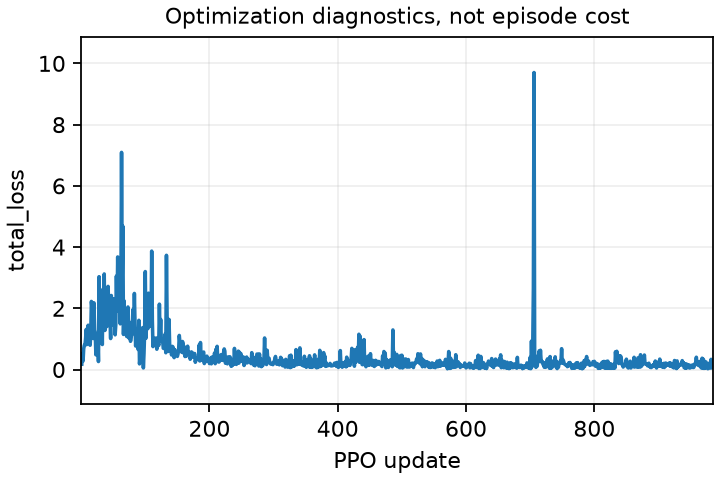
\includegraphics[width=0.25\textwidth,keepaspectratio]{../images/ellipse_500episodes/ppo_loss.png}
    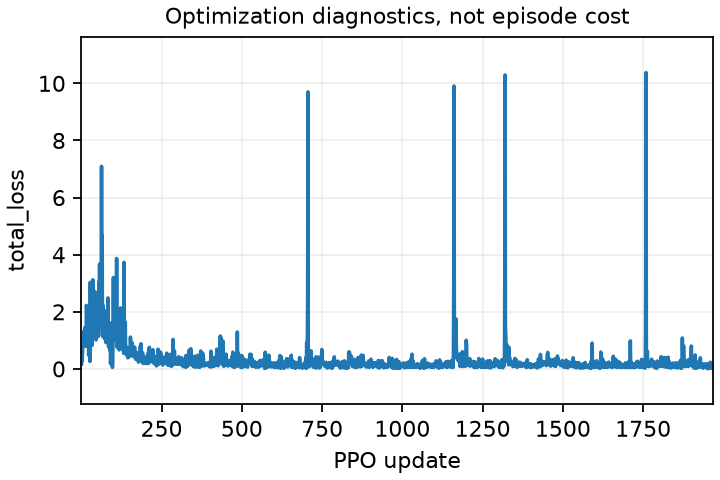
\includegraphics[width=0.25\textwidth,keepaspectratio]{../images/ellipse_1000episodes/ppo_loss.png}
  \end{figure}
\end{frame}

\begin{frame}
  \begin{columns}[T,onlytextwidth]
    \begin{column}{0.5\textwidth}
      \vspace{20pt}
      {\LARGE\bf{AI training TIP}}
      \vspace{20pt}

      \justify
      Irresposible AI training practice could be dangerous not only for your electronic devices but also for you. Watch out because the real terminator doesn't look like the one in the movies!
    \end{column}

    \begin{column}{0.4\textwidth}
      \vspace{10pt}
      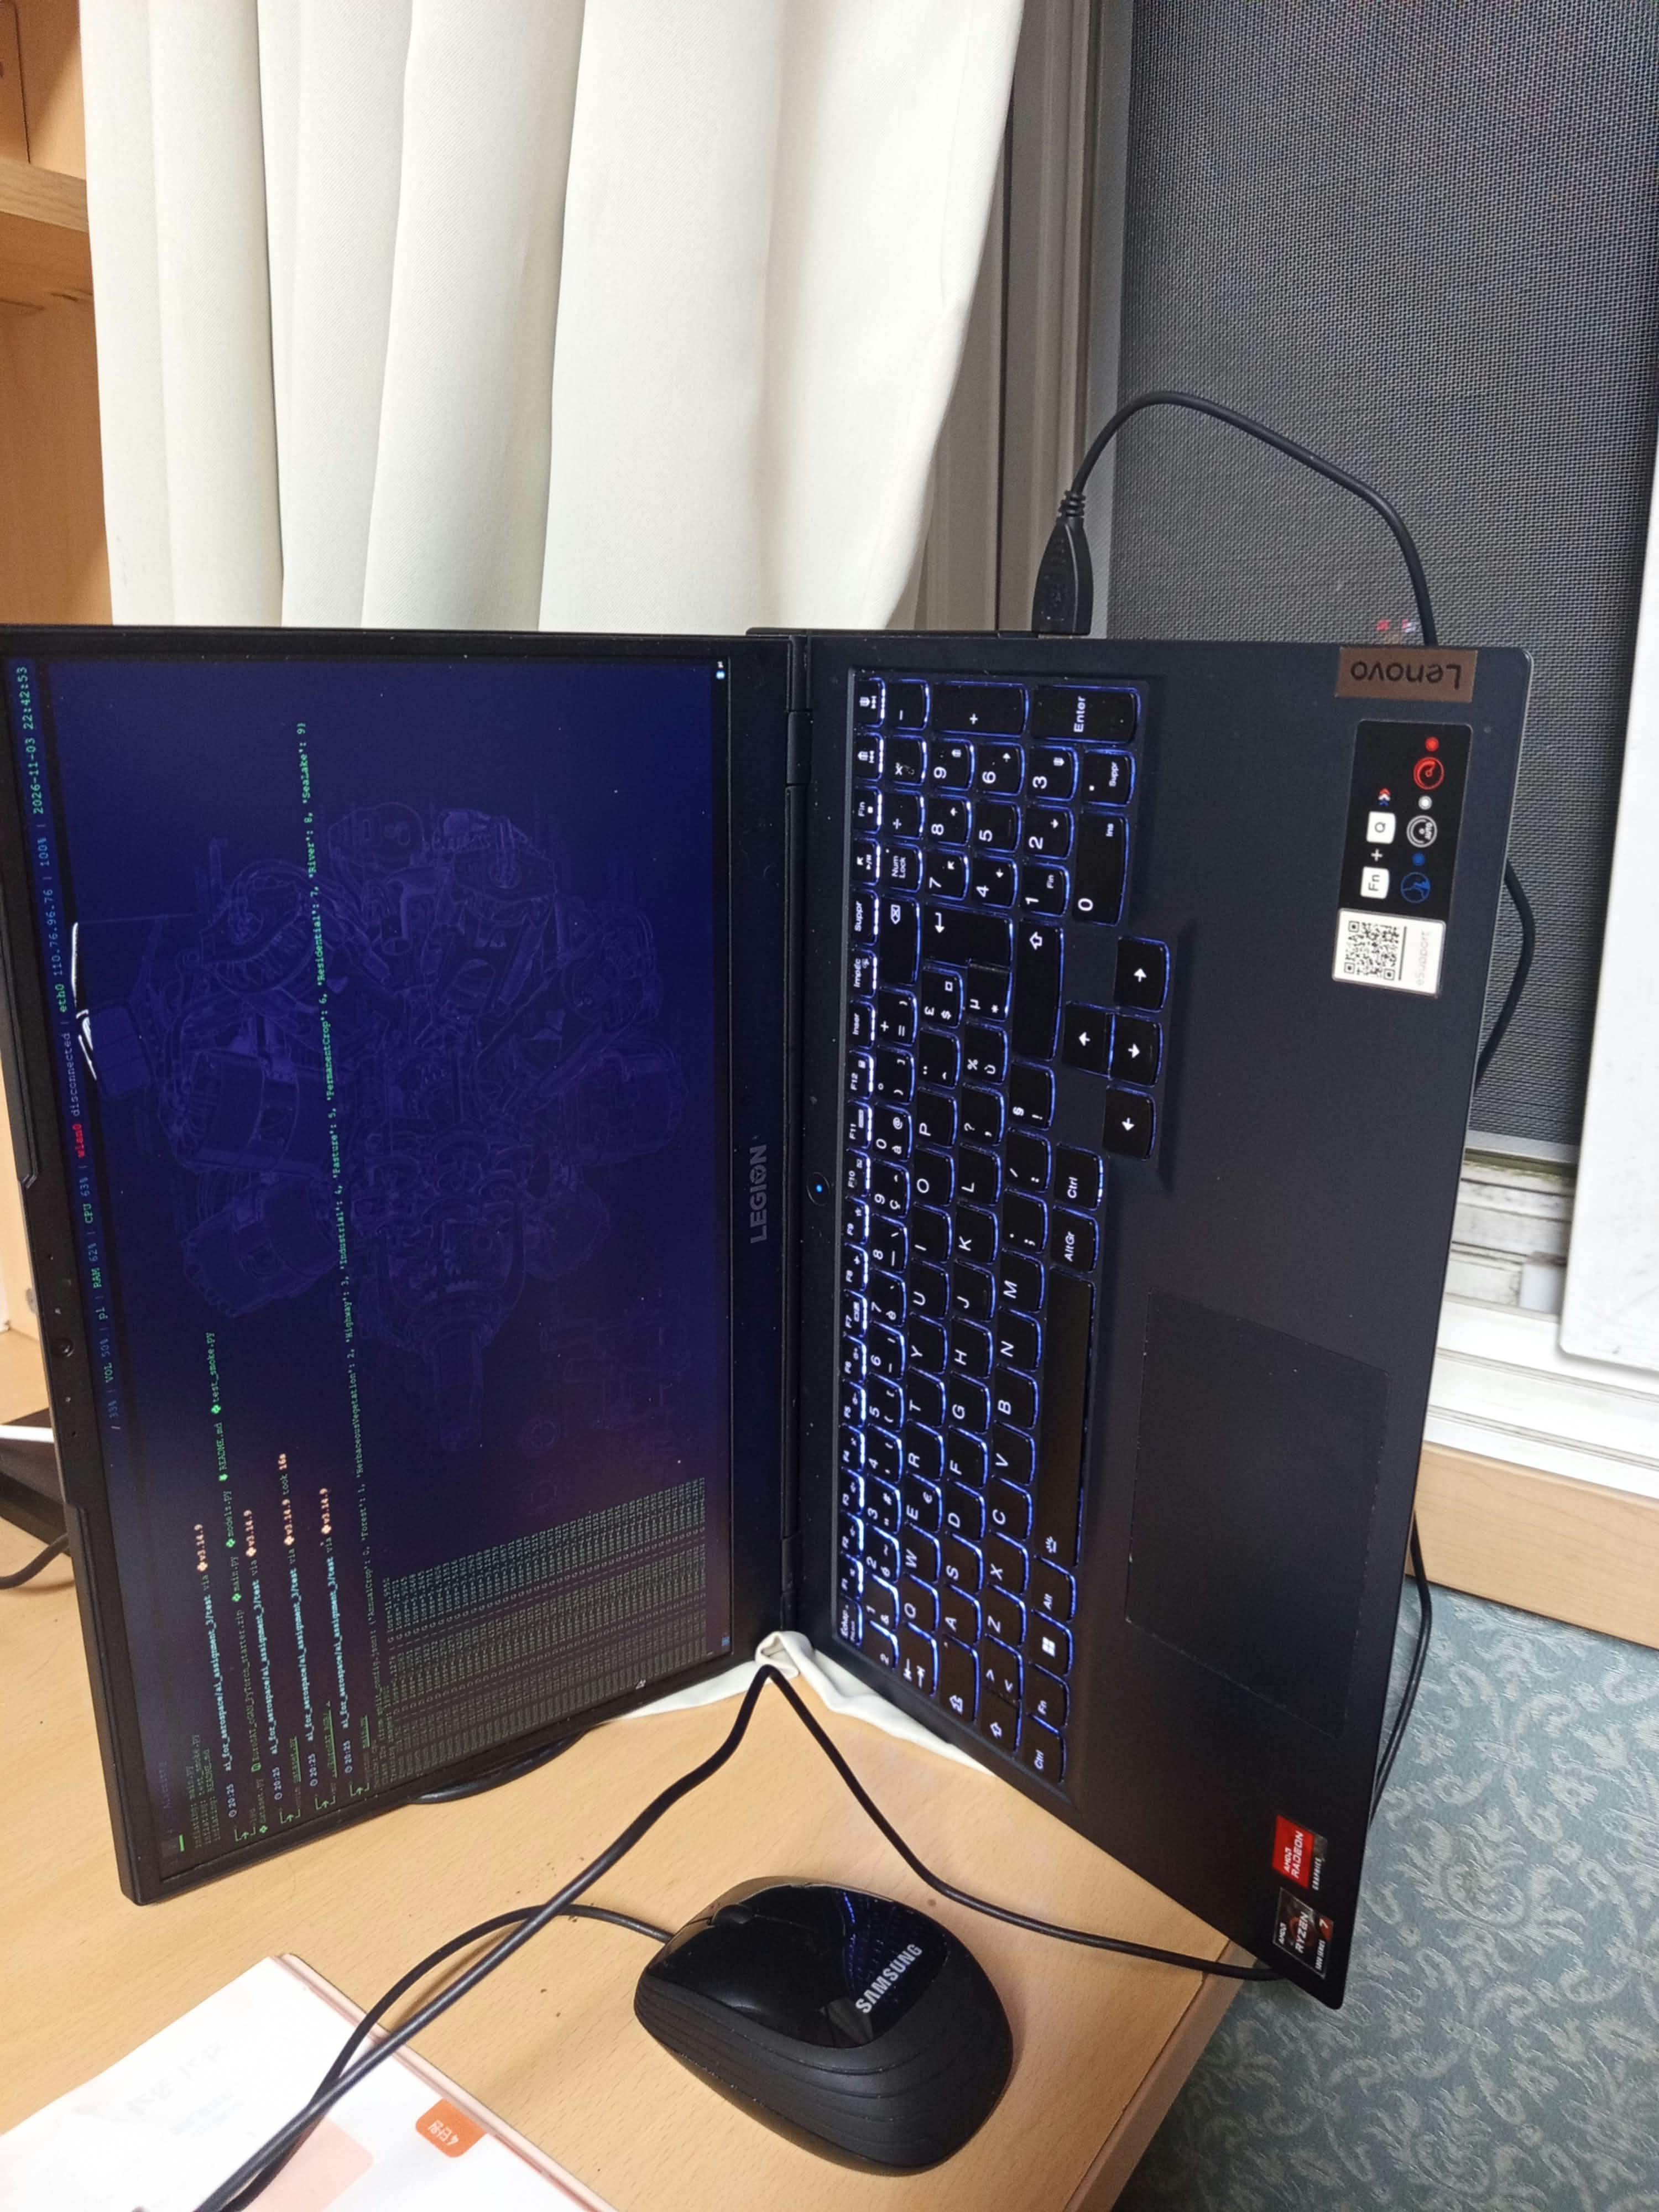
\includegraphics[width=\linewidth, keepaspectratio]{./images/laptop.jpeg}
    \end{column}
  \end{columns}

\end{frame}

\end{document}
